\chapter{Robustness and sensitivity}
\label{ch:ch6}

This chapter assesses the robustness of the profile structure reported in Chapters~\ref{ch:ch4} and~\ref{ch:ch5} along five independent lines. Section~\ref{sec:ch6-algorithms} compares K-means against three agglomerative alternatives. Section~\ref{sec:ch6-duda-hart} reports the Duda--Hart cut-off diagnostics that validate $k = 5$ for Italy and $k = 6$ for Sweden. Section~\ref{sec:ch6-kmeans-lca} compares the K-means assignments with those produced by a Latent Class Analysis. Section~\ref{sec:ch6-fa-stability} evaluates the stability of the factor solution across countries. Section~\ref{sec:ch6-subjective} is the sensitivity analysis that tests the analytical innovation of the thesis: removing the subjective block from the clustering input.

Table~\ref{tab:ch6-profile-sizes} cross-references the profile sizes used throughout the thesis. The Italian total ($n = 2{,}378$) and the Swedish total ($n = 1{,}787$) correspond to the analytical samples after the Mahalanobis screen described in Section~\ref{sec:ch3-sample}.

\begin{table}[ht]
  \centering
  \caption{Profile sizes used throughout the thesis.}
  \label{tab:ch6-profile-sizes}
  \small
  \begin{tabular}{@{}lrr@{}}
    \toprule
    \textbf{Profile} & \textbf{Italy} & \textbf{Sweden}\\
    \midrule
    Fragile Resigned      & 315  & ---  \\
    Fragile Depressed     & 636  & ---  \\
    Moderate Isolated     & 639  & ---  \\
    Traditional Social    & 184  & ---  \\
    Connected Active      & 604  & ---  \\
    \midrule
    Fragile               & ---  & 206  \\
    Social Decline        & ---  & 149  \\
    Moderate              & ---  & 417  \\
    Asset Rich            & ---  & 341  \\
    Wealthy Digital       & ---  & 138  \\
    Connected Wealthy     & ---  & 536  \\
    \midrule
    \textbf{Total}        & \textbf{2{,}378} & \textbf{1{,}787}\\
    \bottomrule
  \end{tabular}
\end{table}

\section{Cluster quality under alternative algorithms}
\label{sec:ch6-algorithms}

The choice of K-means over hierarchical alternatives was motivated in Section~\ref{sec:ch3-kmeans} on theoretical grounds. Figures~\ref{fig:ch6-multi-alg-italy} and~\ref{fig:ch6-multi-alg-sweden} confirm that motivation empirically. Across $k = 2,\ldots,12$ and across the four algorithms considered (K-means, Ward, complete linkage, average linkage), K-means attains uniformly higher within-cluster $R^{2}$ and silhouette than its agglomerative competitors in both countries. Ward linkage is competitive only on the Dunn index, which penalises cluster elongation differently and is known to favour ellipsoidal shapes.

\begin{figure}[ht]
  \centering
  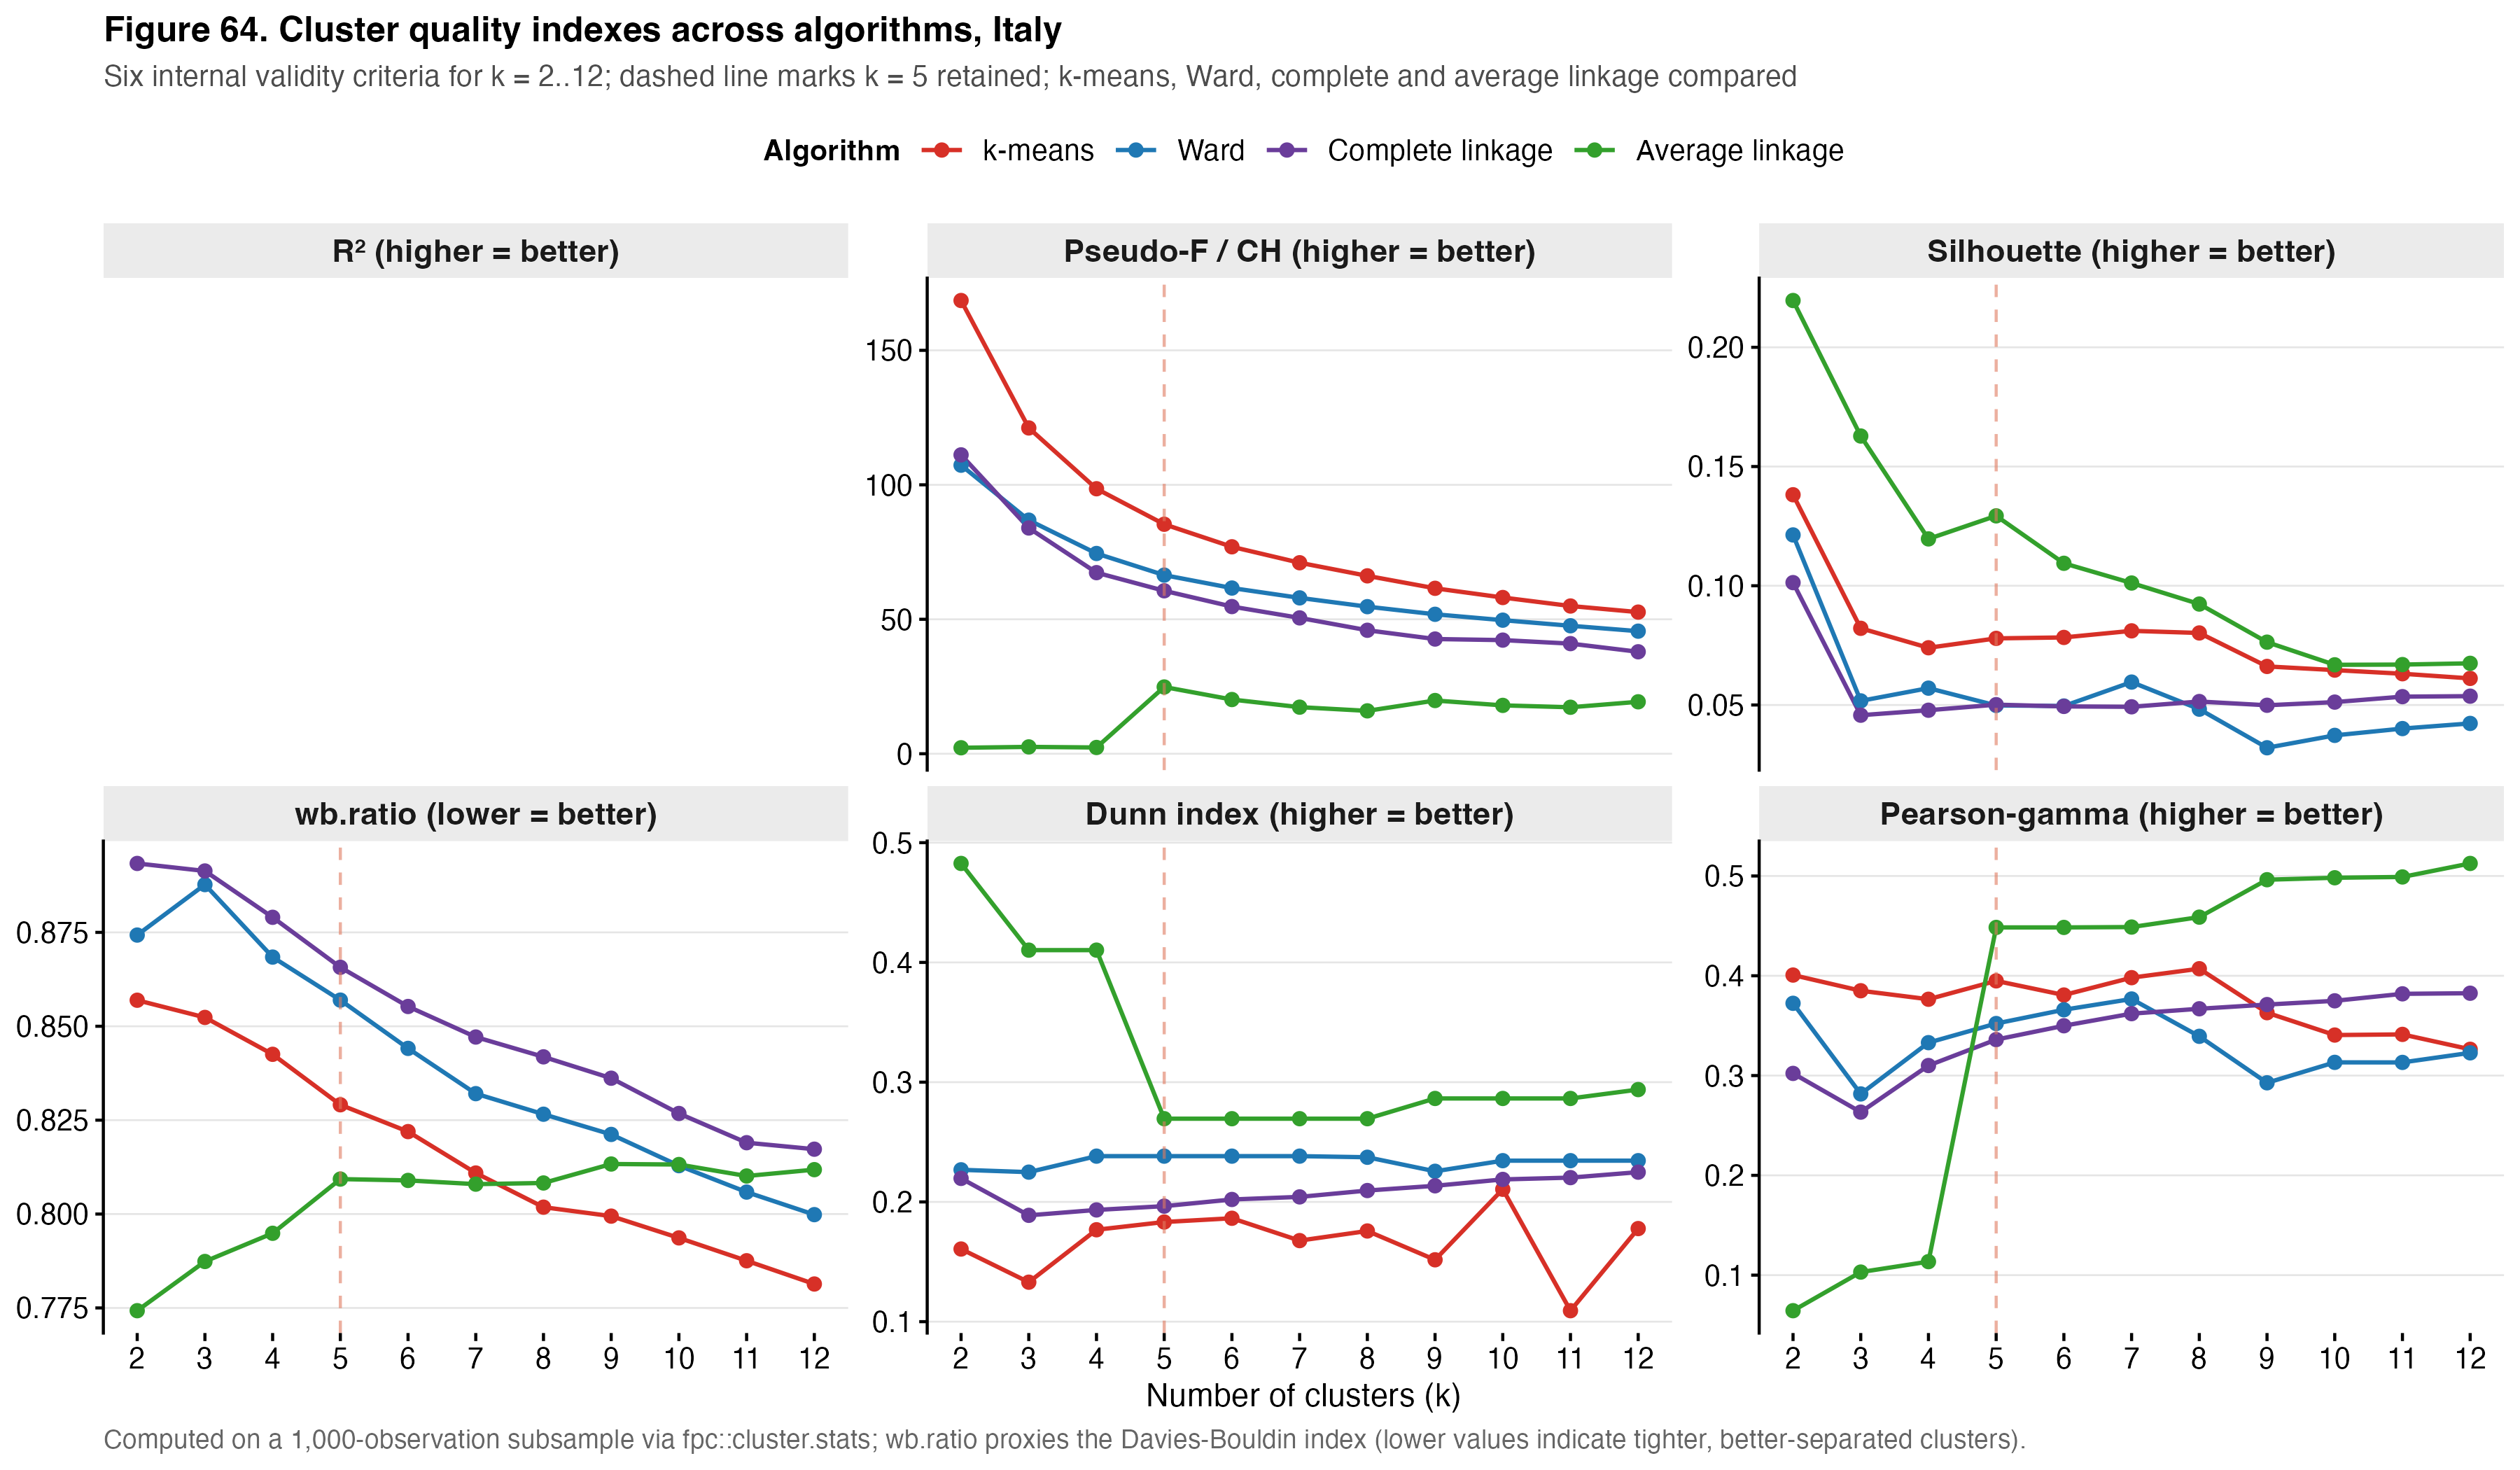
\includegraphics[width=0.92\linewidth]{figures/07_robustness/fig_64_cluster_quality_multi_alg_italy.png}
  \caption{Italy: six internal validity indexes for $k = 2,\ldots,12$ across four clustering algorithms. Source: v9 pipeline.}
  \label{fig:ch6-multi-alg-italy}
\end{figure}

\begin{figure}[ht]
  \centering
  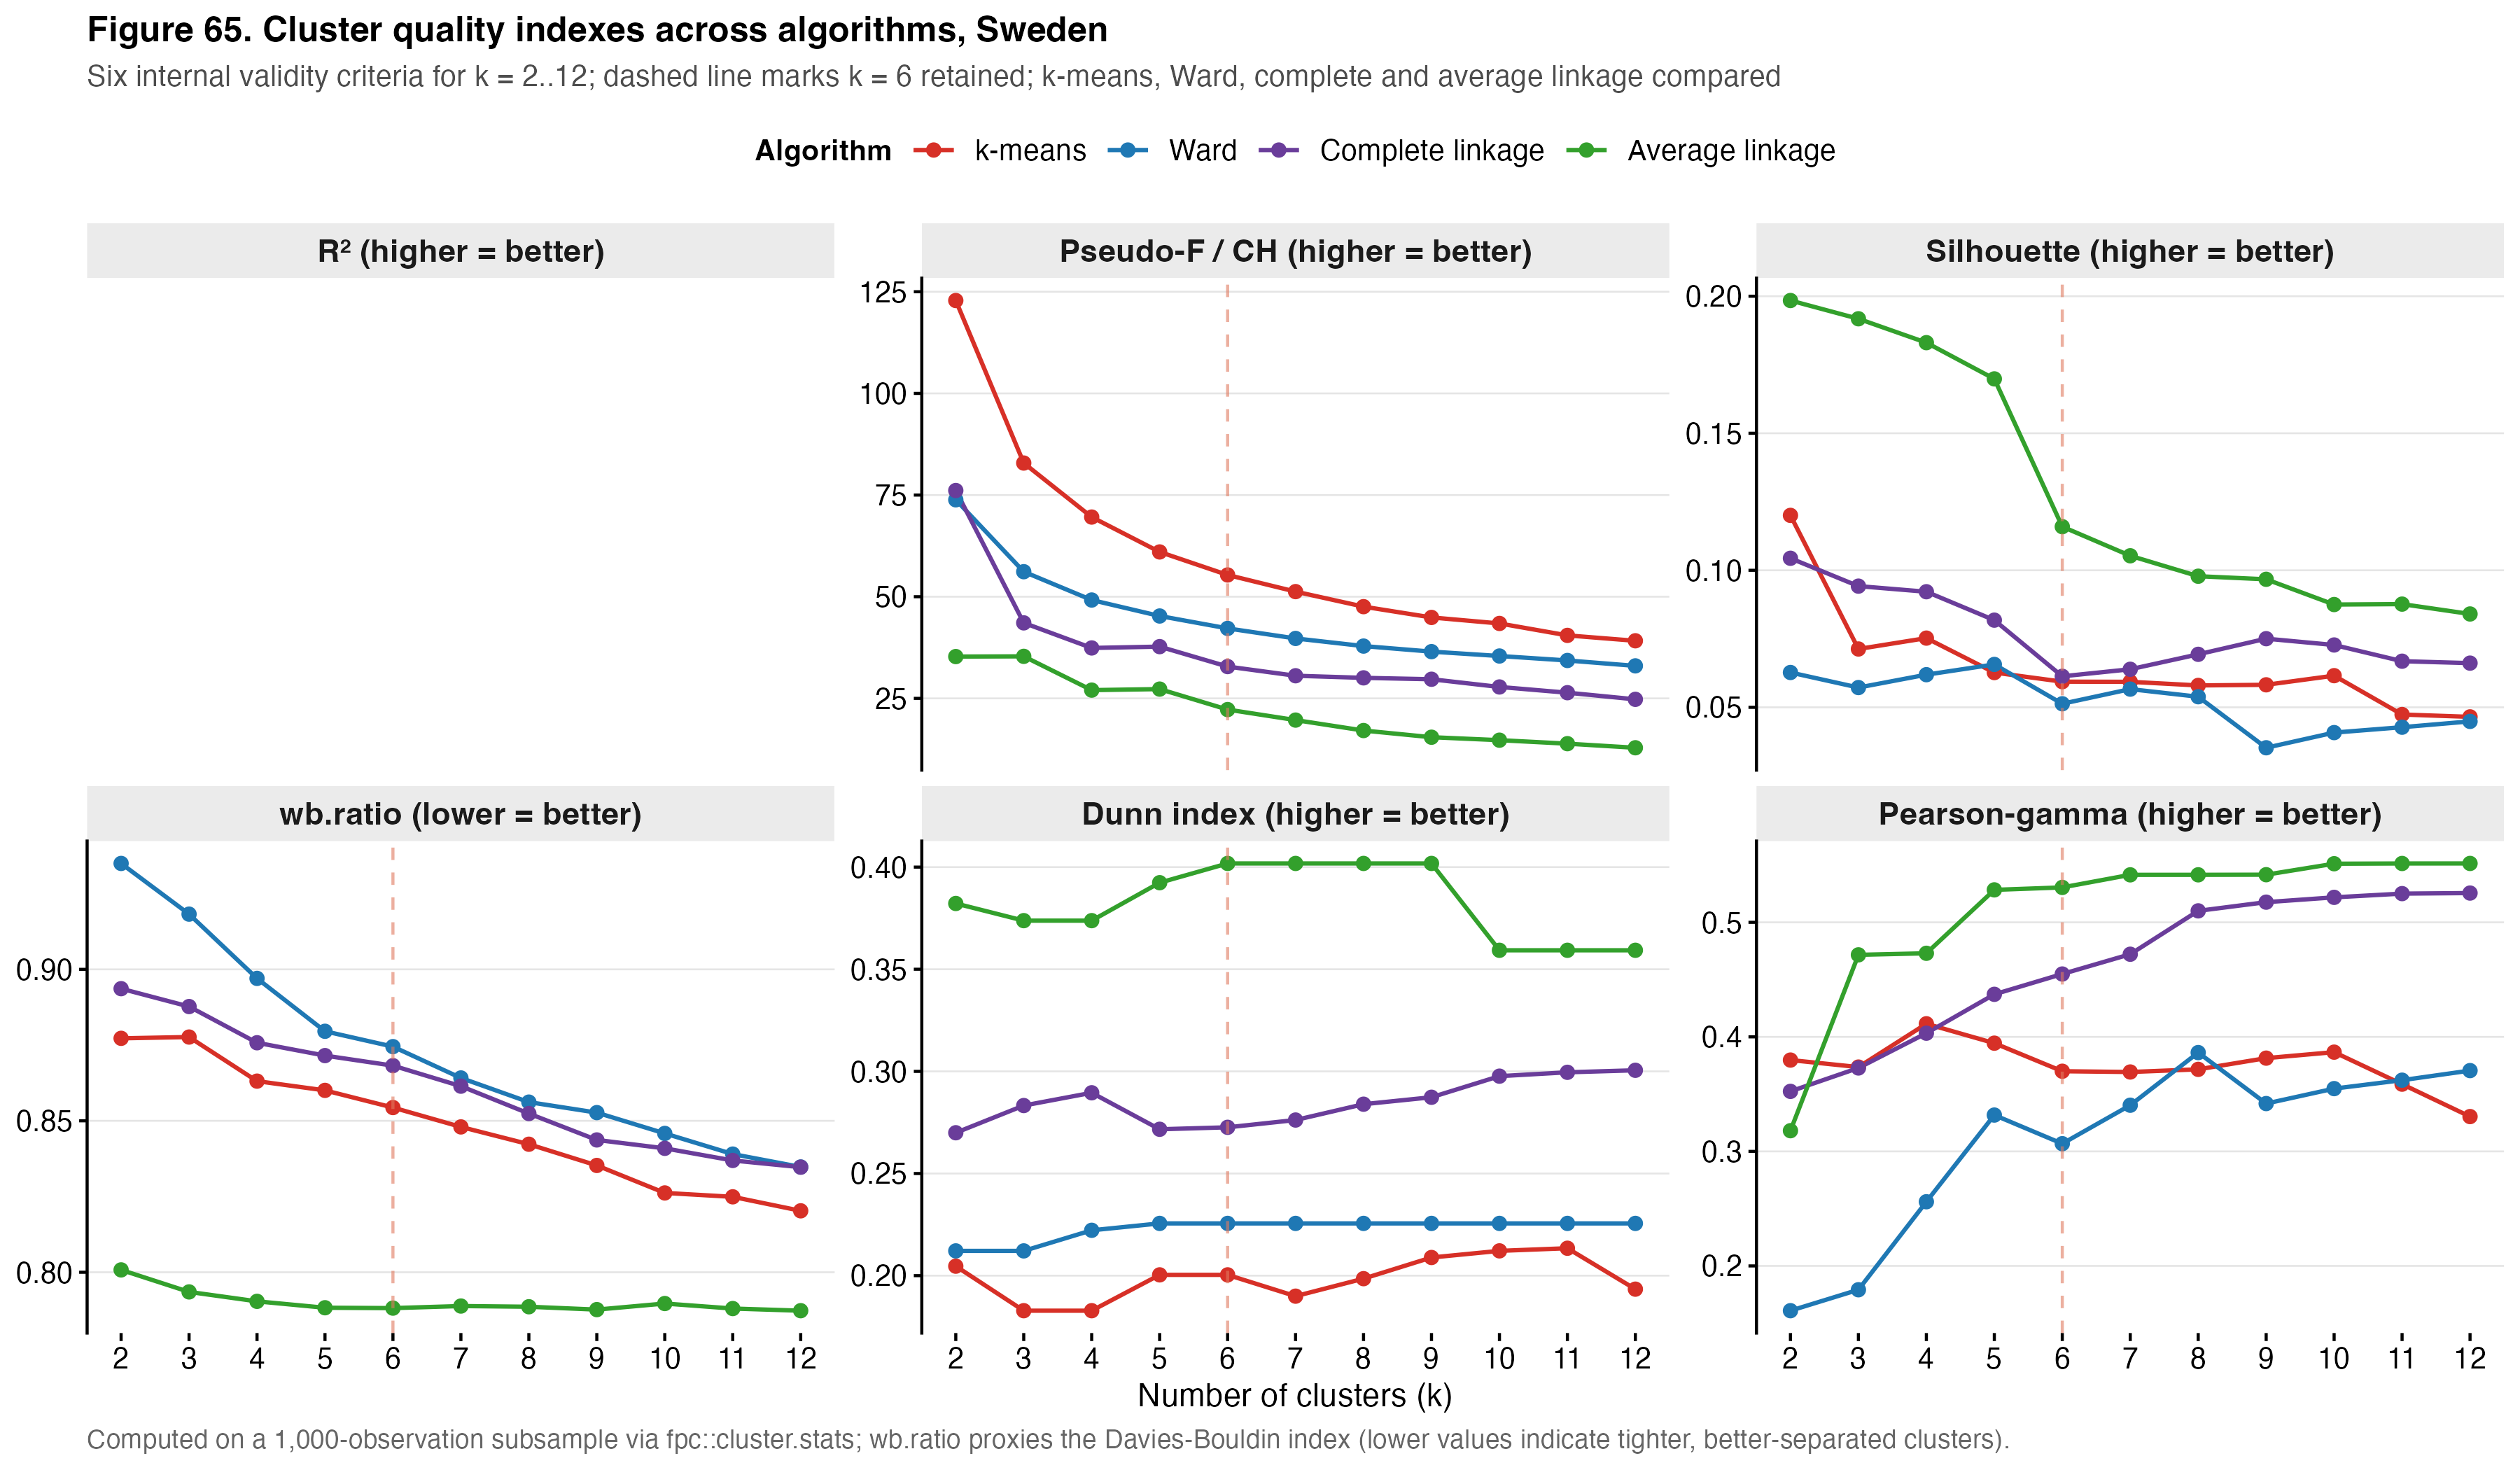
\includegraphics[width=0.92\linewidth]{figures/07_robustness/fig_65_cluster_quality_multi_alg_sweden.png}
  \caption{Sweden: six internal validity indexes for $k = 2,\ldots,12$ across four clustering algorithms. Source: v9 pipeline.}
  \label{fig:ch6-multi-alg-sweden}
\end{figure}

Figures~\ref{fig:ch6-varspec-italy} and~\ref{fig:ch6-varspec-sweden} report, variable by variable, the within-cluster $R^{2}$ attained by each algorithm at each $k$. Two interpretive patterns emerge. First, a small group of indicators --- notably \emph{bmi} and \emph{received help} (\emph{sp002\_}) --- carries no clustering signal under any method at any $k$; these variables are retained because the thesis's methodological choice is to refrain from ad-hoc variable pruning, but the reader is alerted that their contribution to the partition is nil. Second, the bulk of the indicators saturate their within-cluster $R^{2}$ precisely in the $k = 5,\ldots,6$ range, which converges with the empirical and substantive choice of $k = 5$ for Italy and $k = 6$ for Sweden.

\begin{figure}[ht]
  \centering
  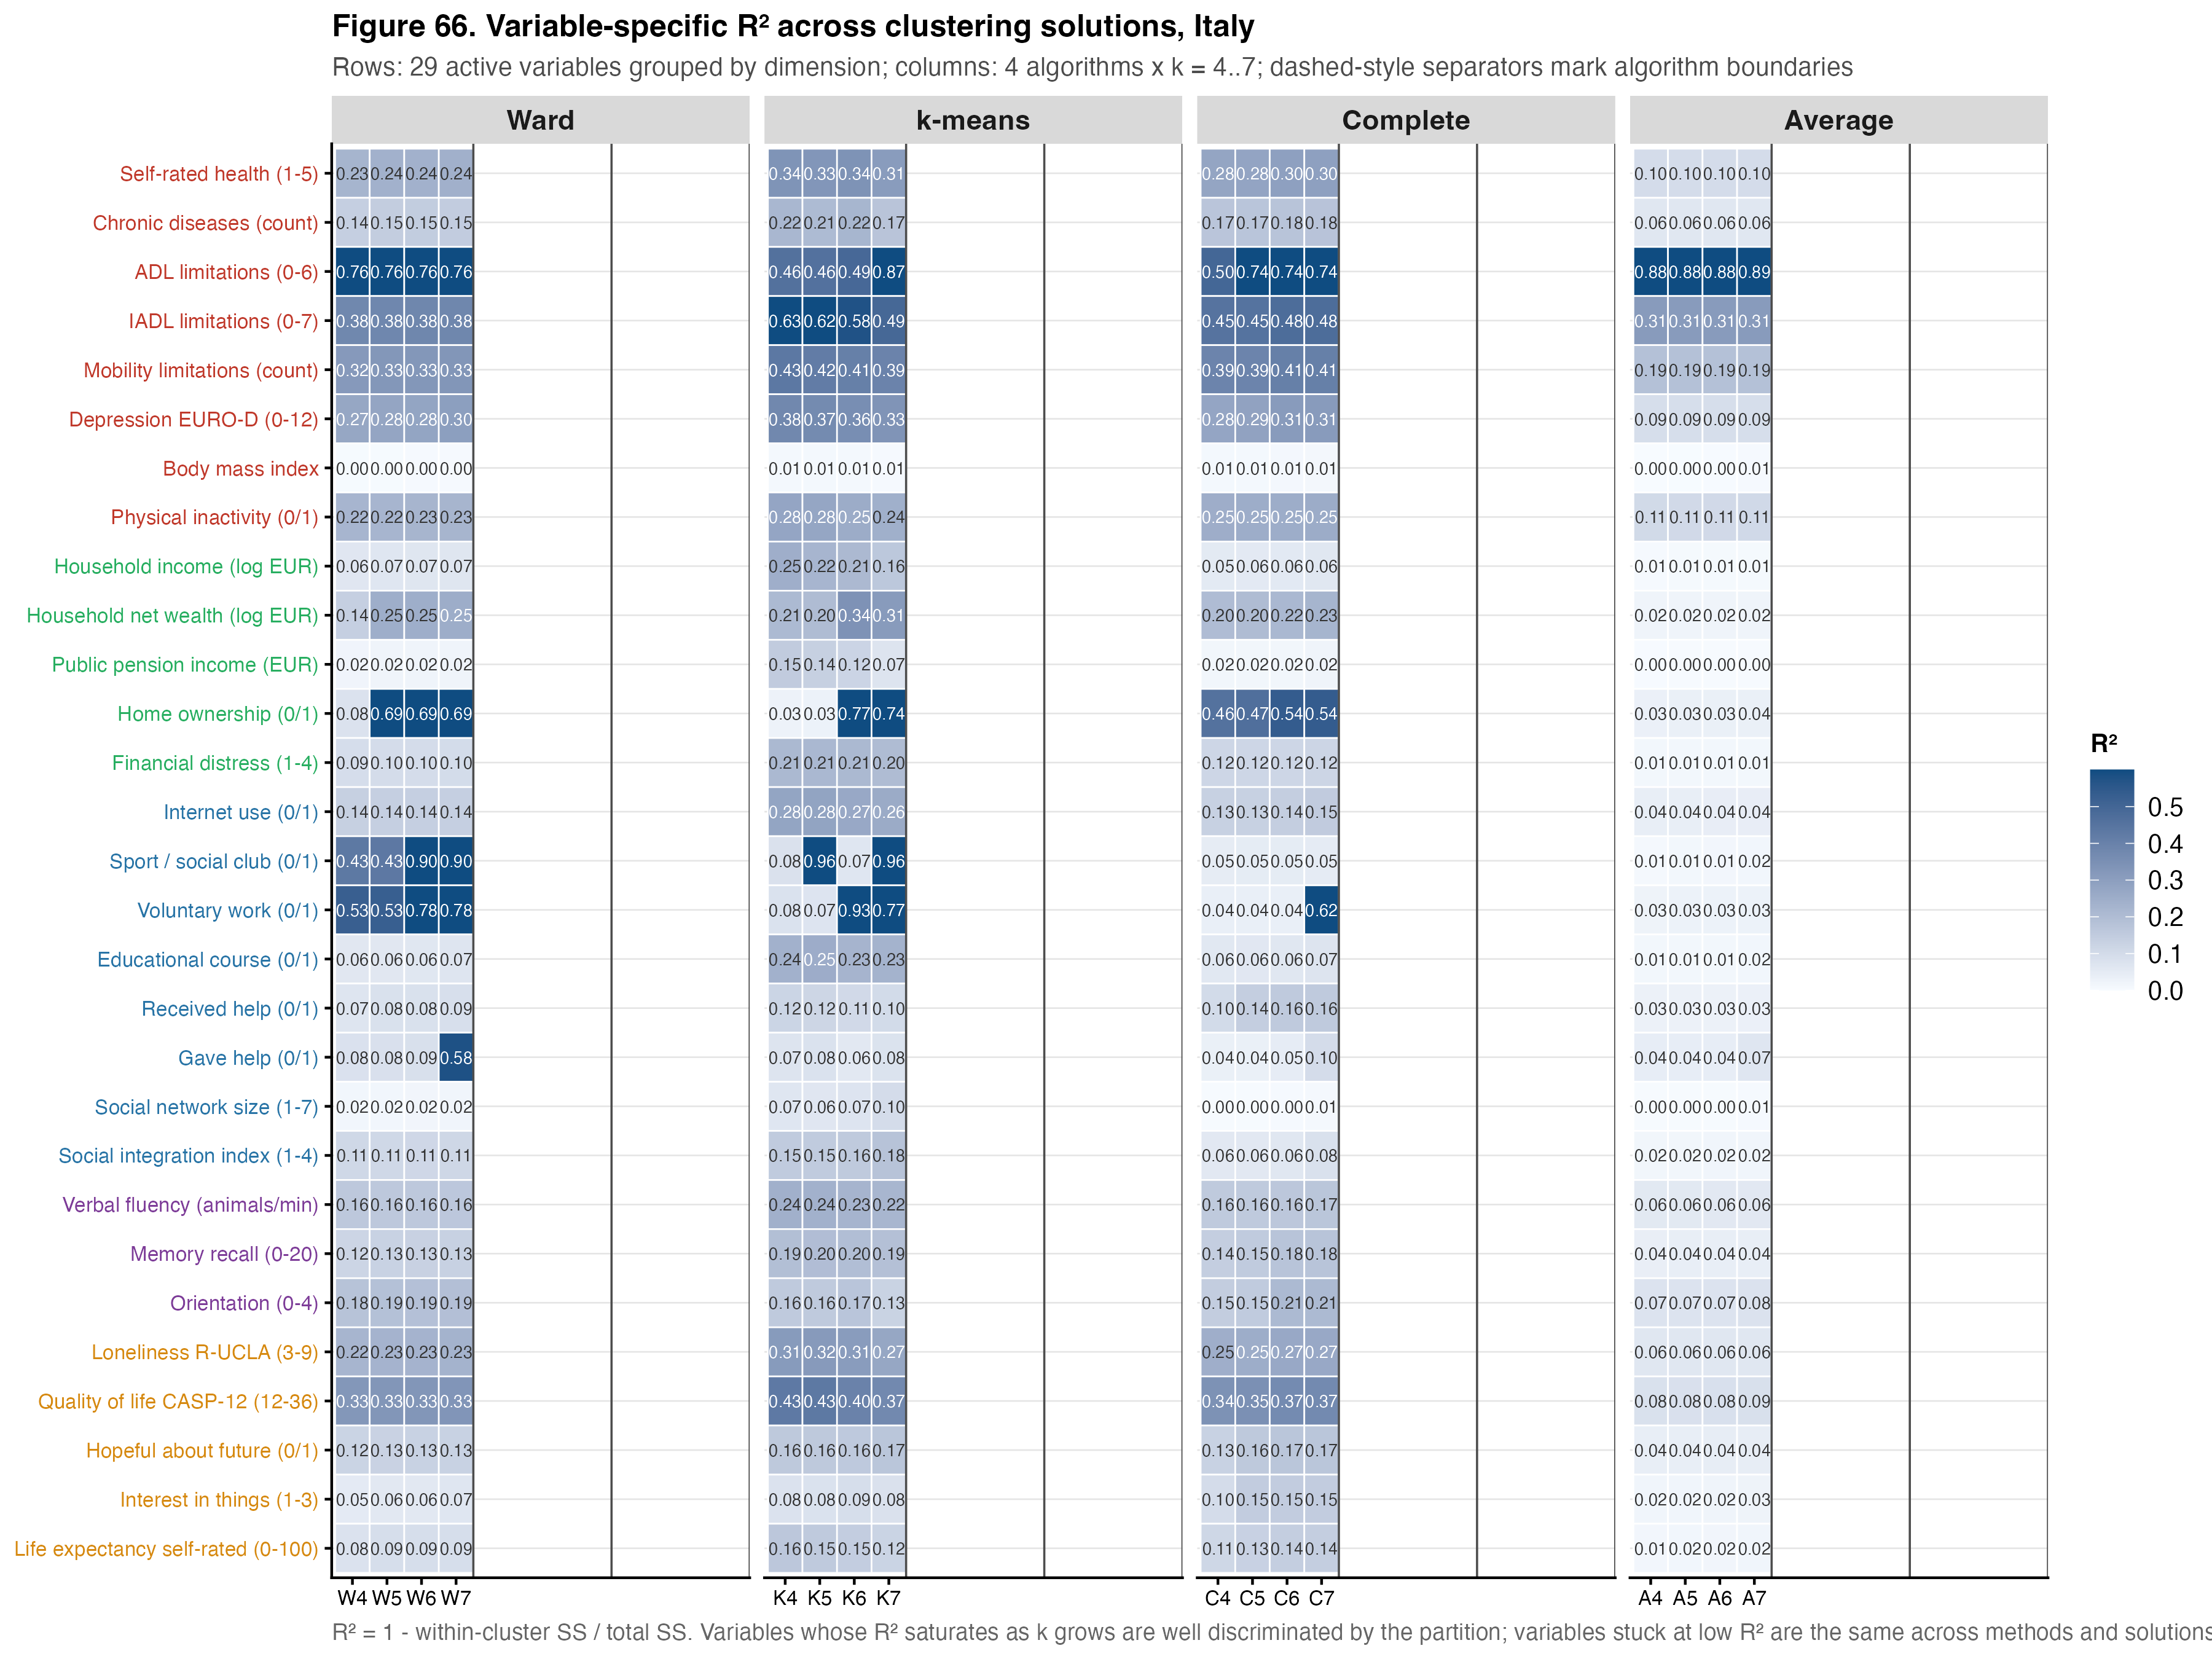
\includegraphics[width=0.92\linewidth]{figures/07_robustness/fig_66_varspec_r2_italy.png}
  \caption{Italy: variable-specific within-cluster $R^{2}$ across clustering solutions. Source: v9 pipeline.}
  \label{fig:ch6-varspec-italy}
\end{figure}

\begin{figure}[ht]
  \centering
  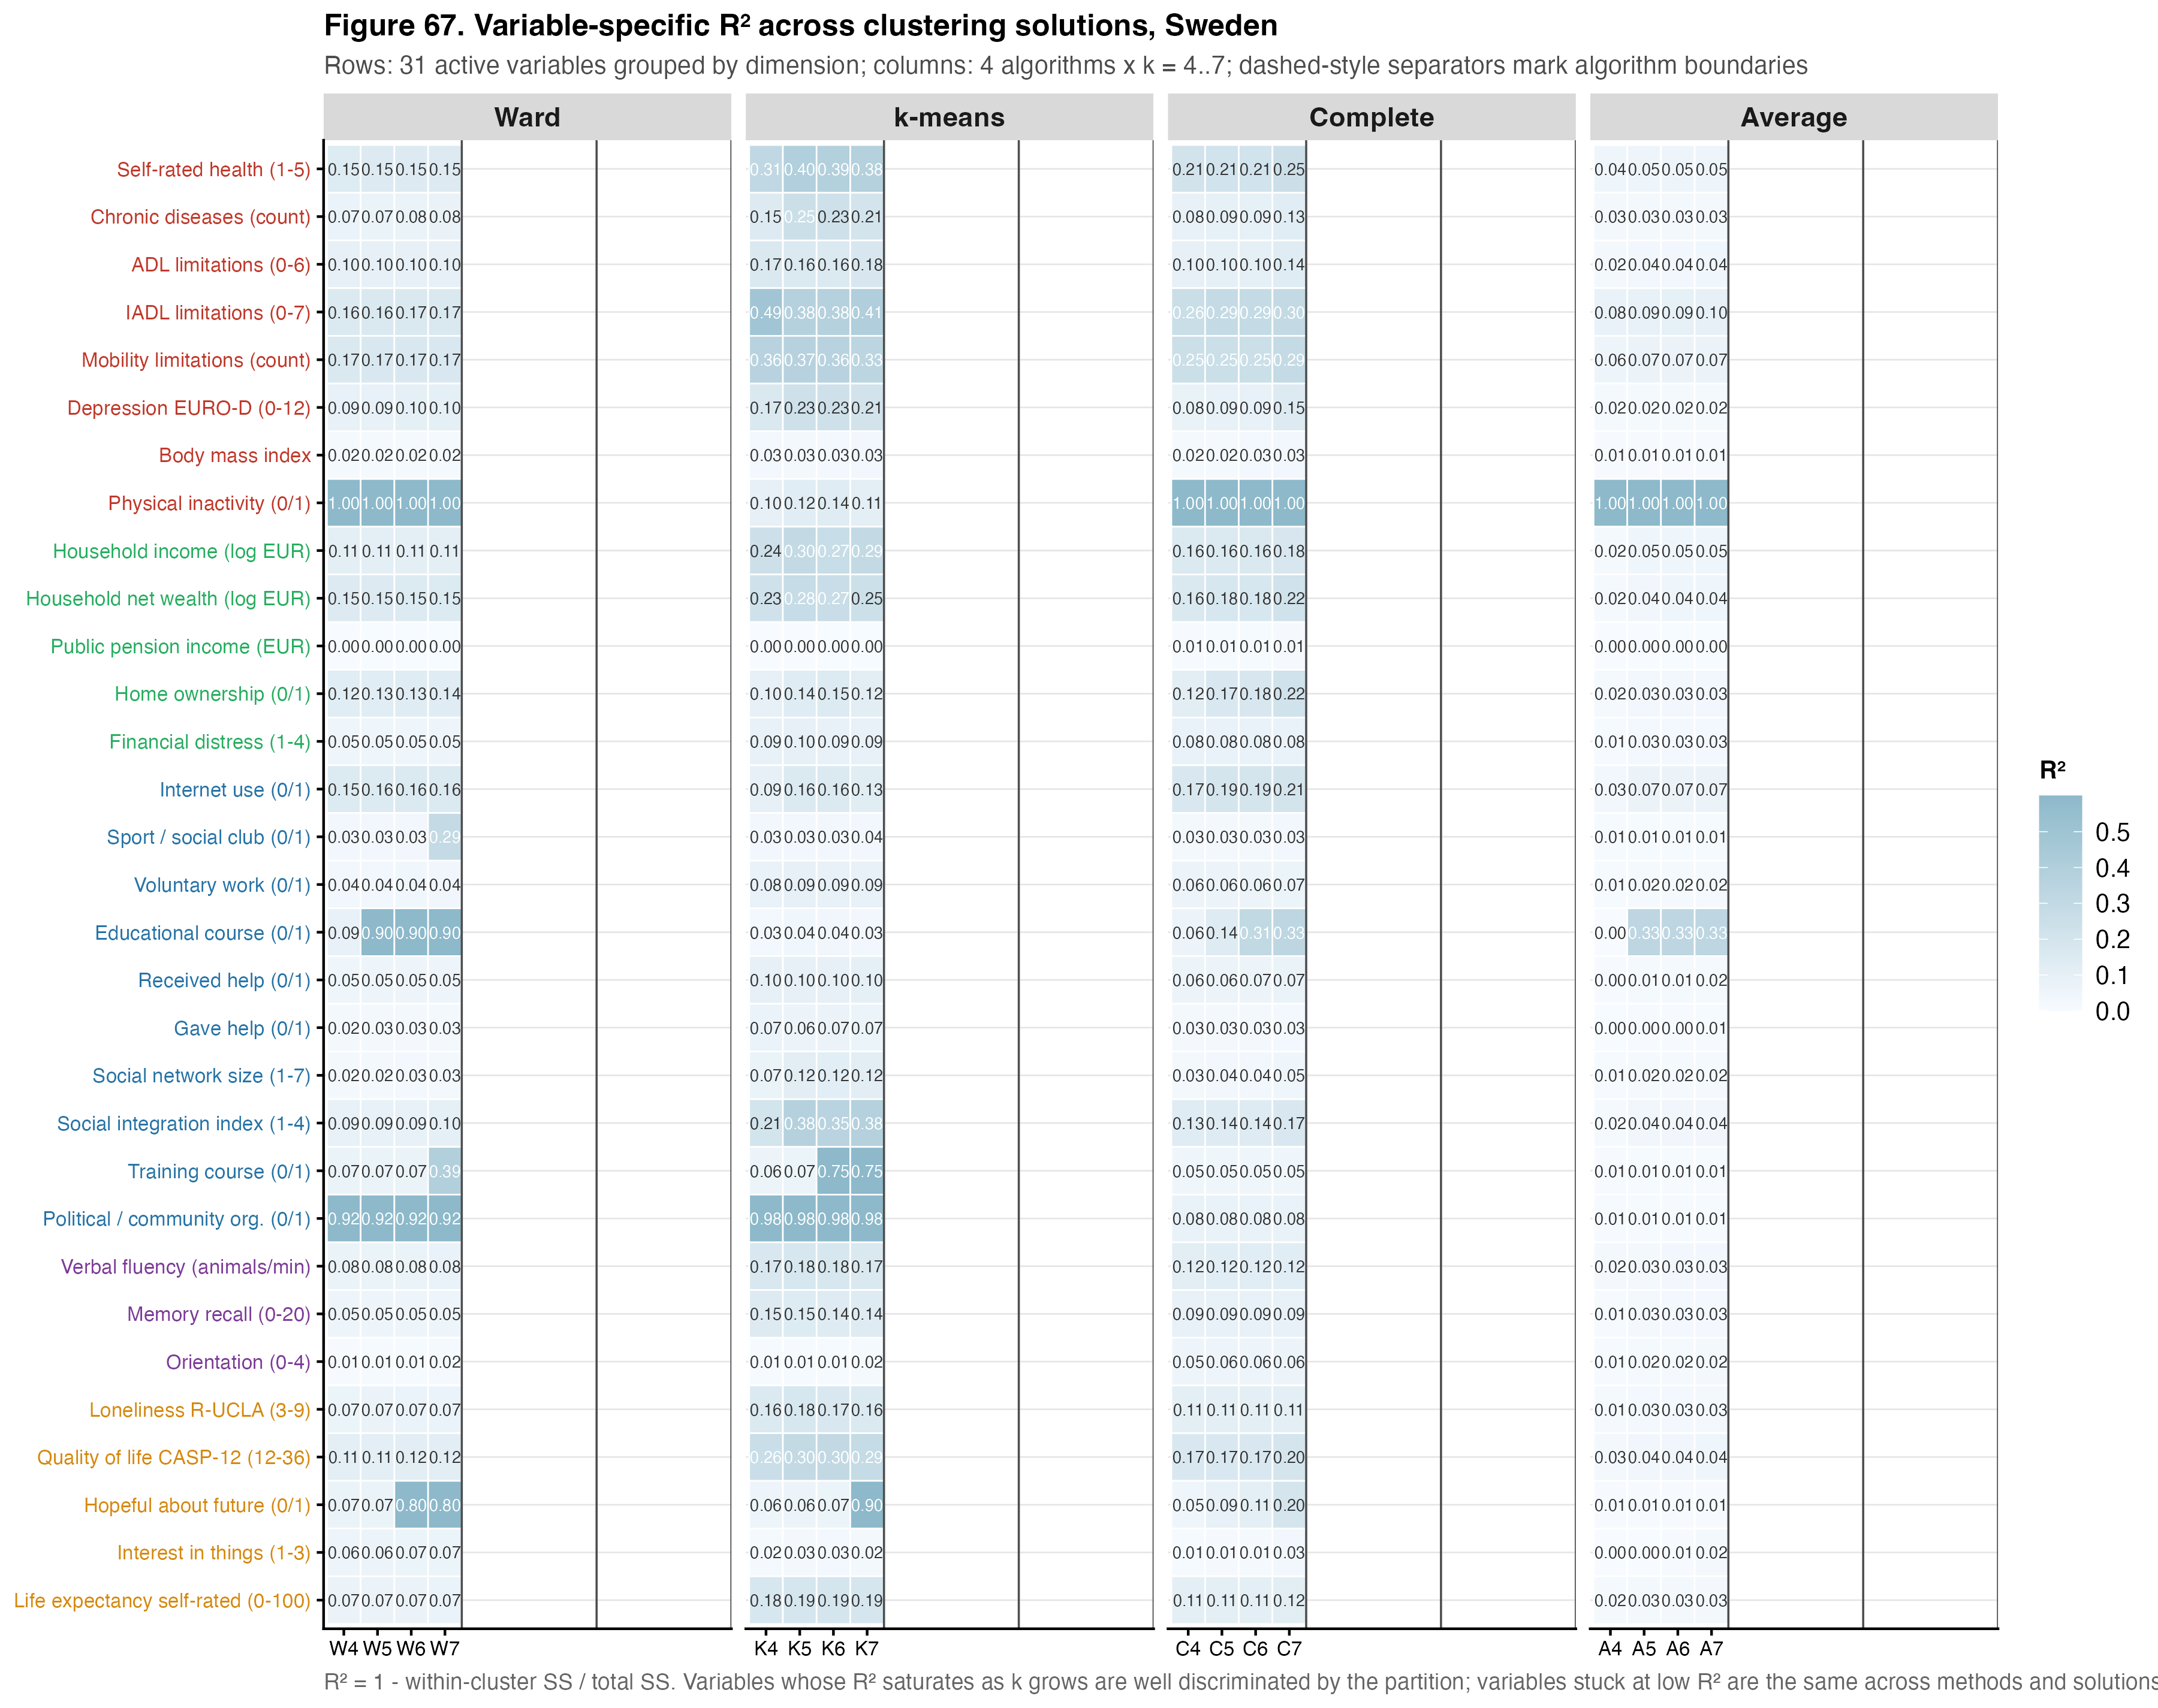
\includegraphics[width=0.92\linewidth]{figures/07_robustness/fig_67_varspec_r2_sweden.png}
  \caption{Sweden: variable-specific within-cluster $R^{2}$ across clustering solutions. Source: v9 pipeline.}
  \label{fig:ch6-varspec-sweden}
\end{figure}

\section{Hierarchical cut-off diagnostics (Duda--Hart)}
\label{sec:ch6-duda-hart}

Figures~\ref{fig:ch6-sprt2-italy} and~\ref{fig:ch6-sprt2-sweden} report the semi-partial $R^{2}$ (SPR$^{2}$) and the Pseudo-$T^{2}$ (PST$^{2}$) diagnostics of Duda and Hart for the three agglomerative linkages across $k = 2,\ldots,12$. These curves identify the "merge cost" at each level of the hierarchy: a peak in PST$^{2}$ or a sharp jump in SPR$^{2}$ at $k = k^{*}$ signals that collapsing two clusters at that level destroys a well-separated group, which is the classical criterion for cutting the tree at $k^{*}$.

\begin{figure}[ht]
  \centering
  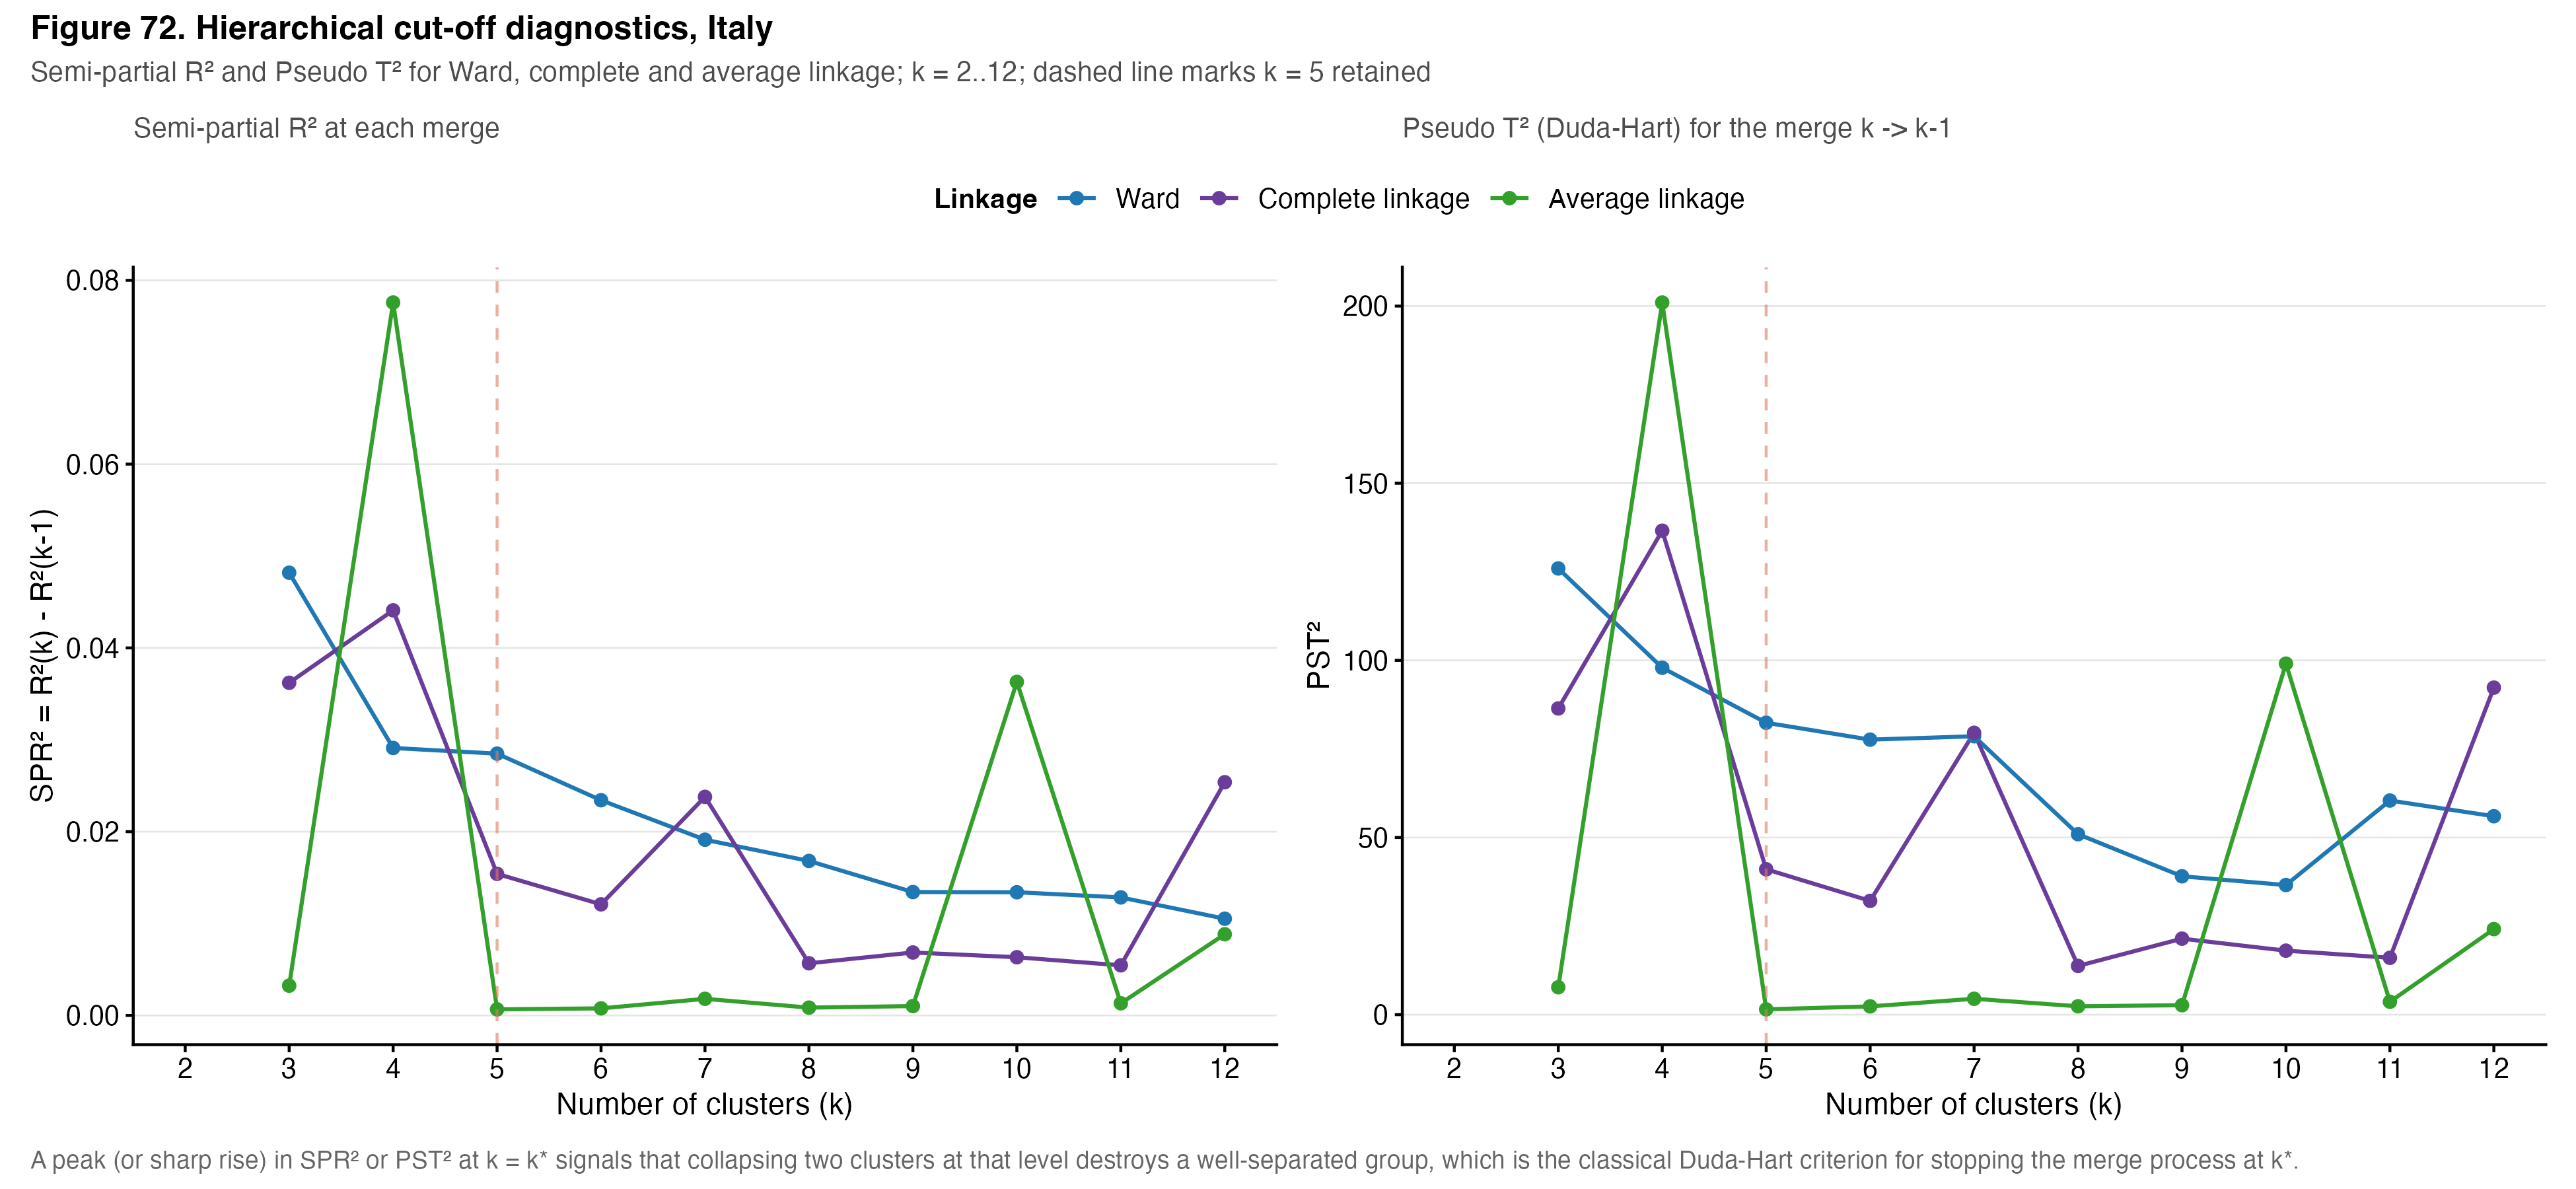
\includegraphics[width=0.92\linewidth]{figures/08_appendix/fig_72_spr2_pst2_italy.png}
  \caption{Italy: semi-partial $R^{2}$ and Pseudo-$T^{2}$ for Ward, complete, and average linkage. Dashed line marks $k = 5$. Source: v9 pipeline.}
  \label{fig:ch6-sprt2-italy}
\end{figure}

\begin{figure}[ht]
  \centering
  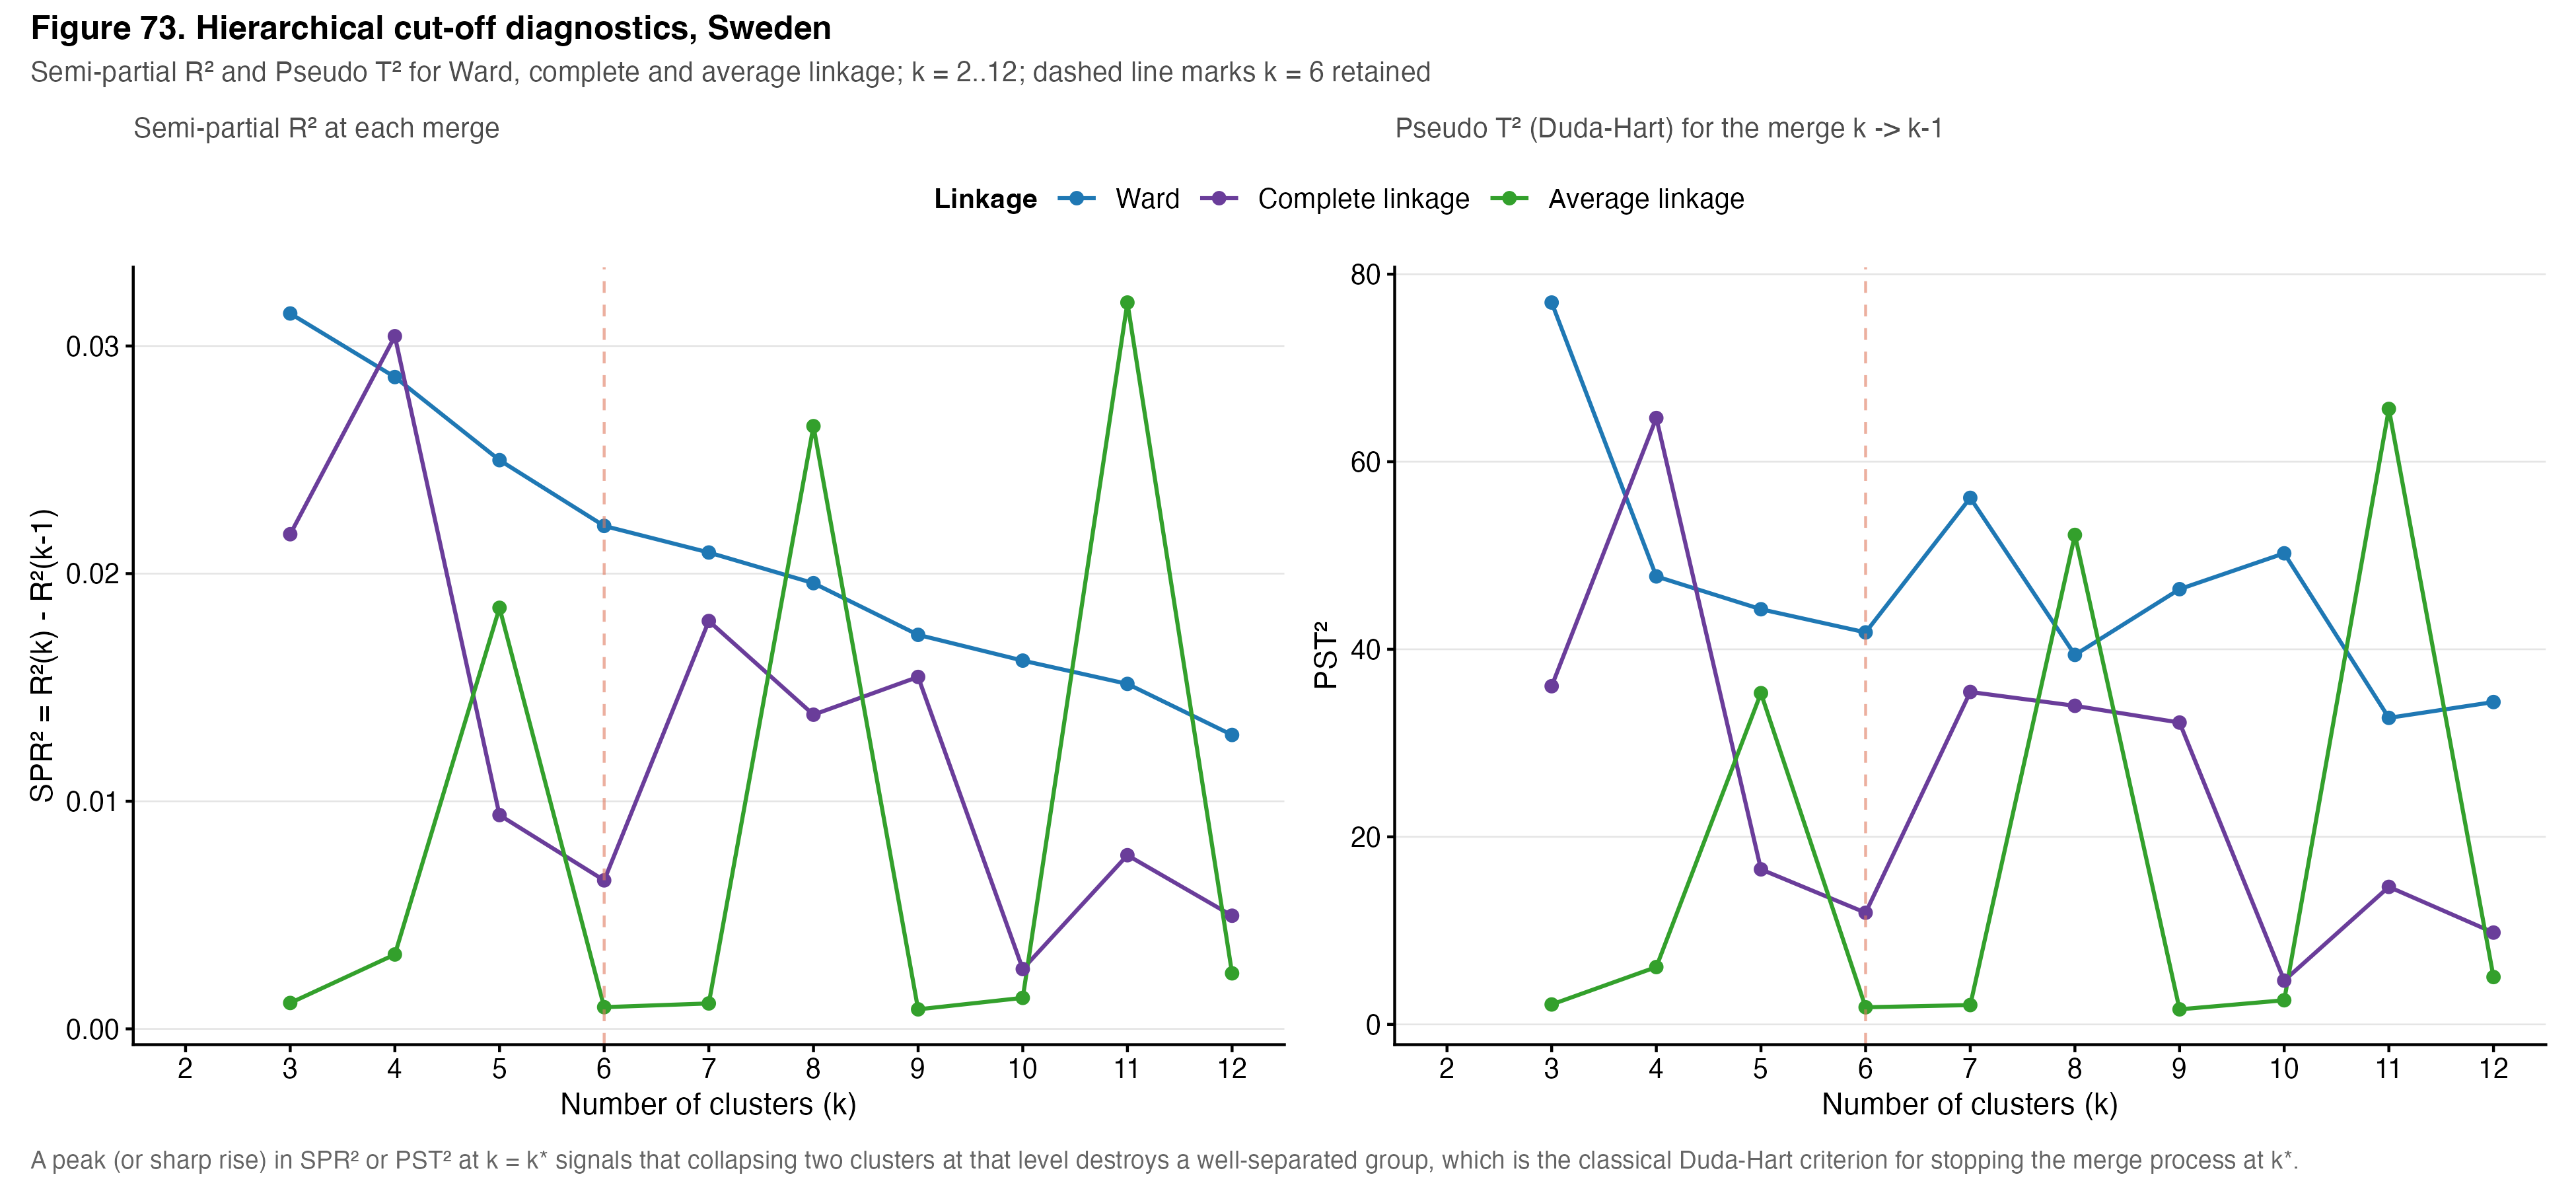
\includegraphics[width=0.92\linewidth]{figures/08_appendix/fig_73_spr2_pst2_sweden.png}
  \caption{Sweden: semi-partial $R^{2}$ and Pseudo-$T^{2}$ for Ward, complete, and average linkage. Dashed line marks $k = 6$. Source: v9 pipeline.}
  \label{fig:ch6-sprt2-sweden}
\end{figure}

The peaks of PST$^{2}$ for Ward linkage fall at $k = 5$ in Italy and at $k = 6$ in Sweden, independently corroborating the cut-off chosen for the K-means solution. On average and complete linkage the peaks are less sharp, consistent with the known tendency of those methods to produce shallower dendrogram structures under mixed-scale data.

\section{Convergence between K-means and Latent Class Analysis}
\label{sec:ch6-kmeans-lca}

Latent Class Analysis provides a probabilistic alternative to the distance-based K-means. Convergence between the two is the most stringent internal robustness check, because the two methods rest on different theoretical premises: K-means minimises the within-cluster sum of squares under a hard-assignment, equal-variance Gaussian assumption, while LCA models the joint distribution of the (discretised) indicators as a mixture of multinomials and yields posterior class probabilities.

Figures~\ref{fig:ch6-lca-fit}, \ref{fig:ch6-lca-confusion} and~\ref{fig:ch6-convergence} summarise the result. The BIC of LCA is minimised at $k = 6$ for both countries, matching the $k$ retained in the K-means stage. Normalised entropy of the LCA posterior is $0.83$ in Italy and in Sweden, above the conventional 0.80 threshold for adequate classification quality. The confusion matrices between K-means and the modal LCA class show that the majority of respondents land in the same class under both methods.

\begin{figure}[ht]
  \centering
  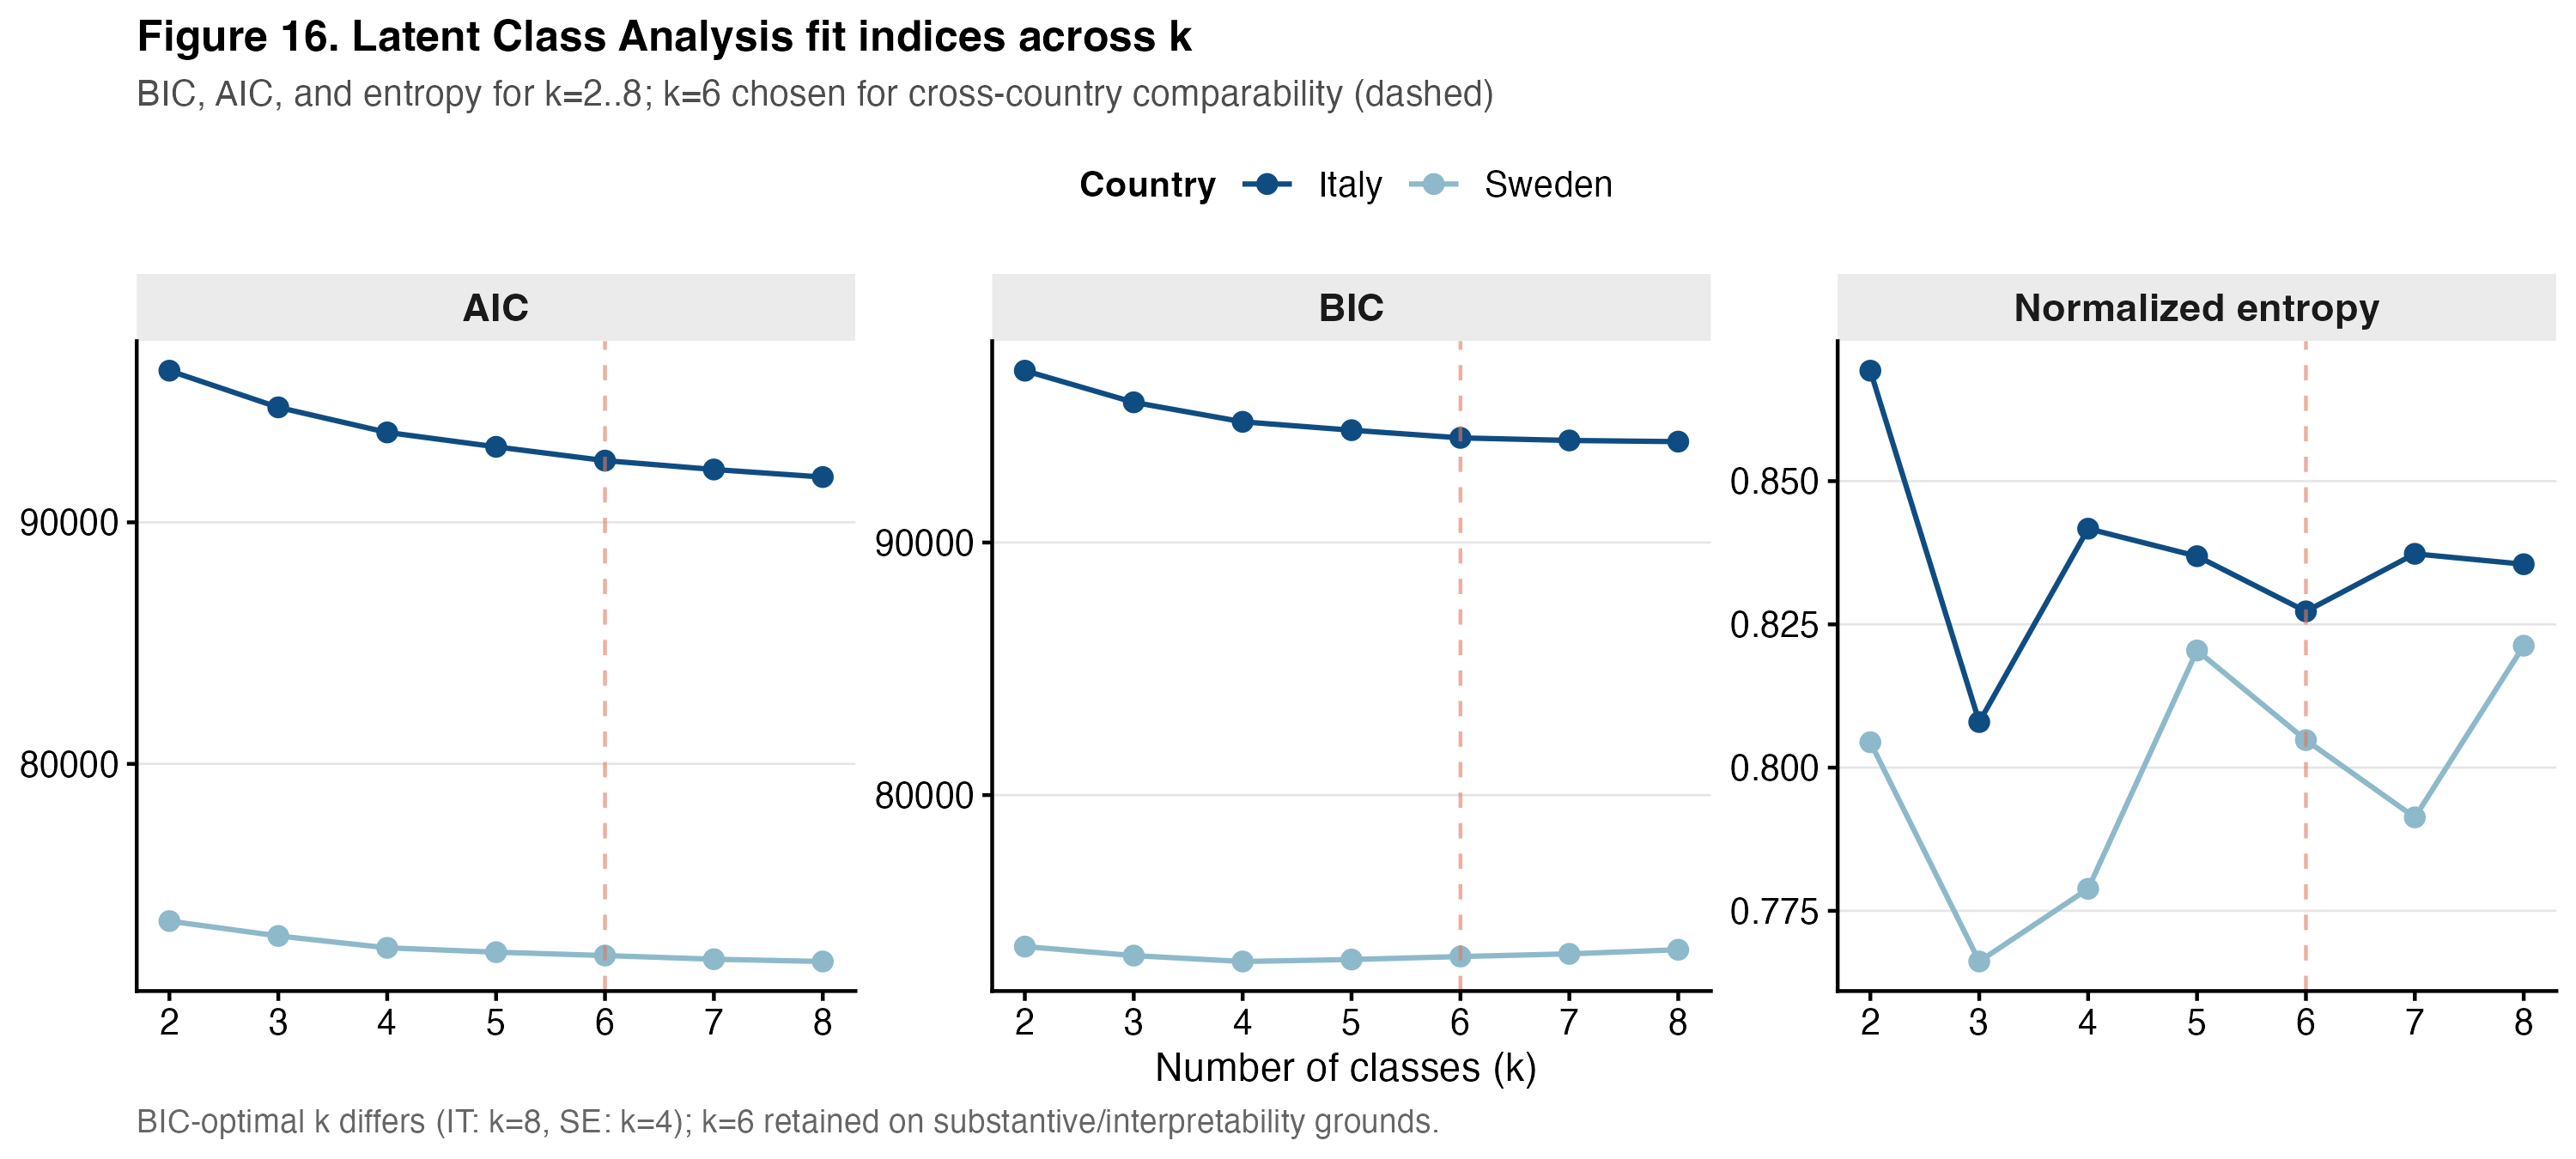
\includegraphics[width=0.82\linewidth]{figures/07_robustness/fig_16_lca_fit_indices.png}
  \caption{LCA model fit indices for Italy and Sweden across $k = 2,\ldots,8$. Source: v9 pipeline.}
  \label{fig:ch6-lca-fit}
\end{figure}

\begin{figure}[ht]
  \centering
  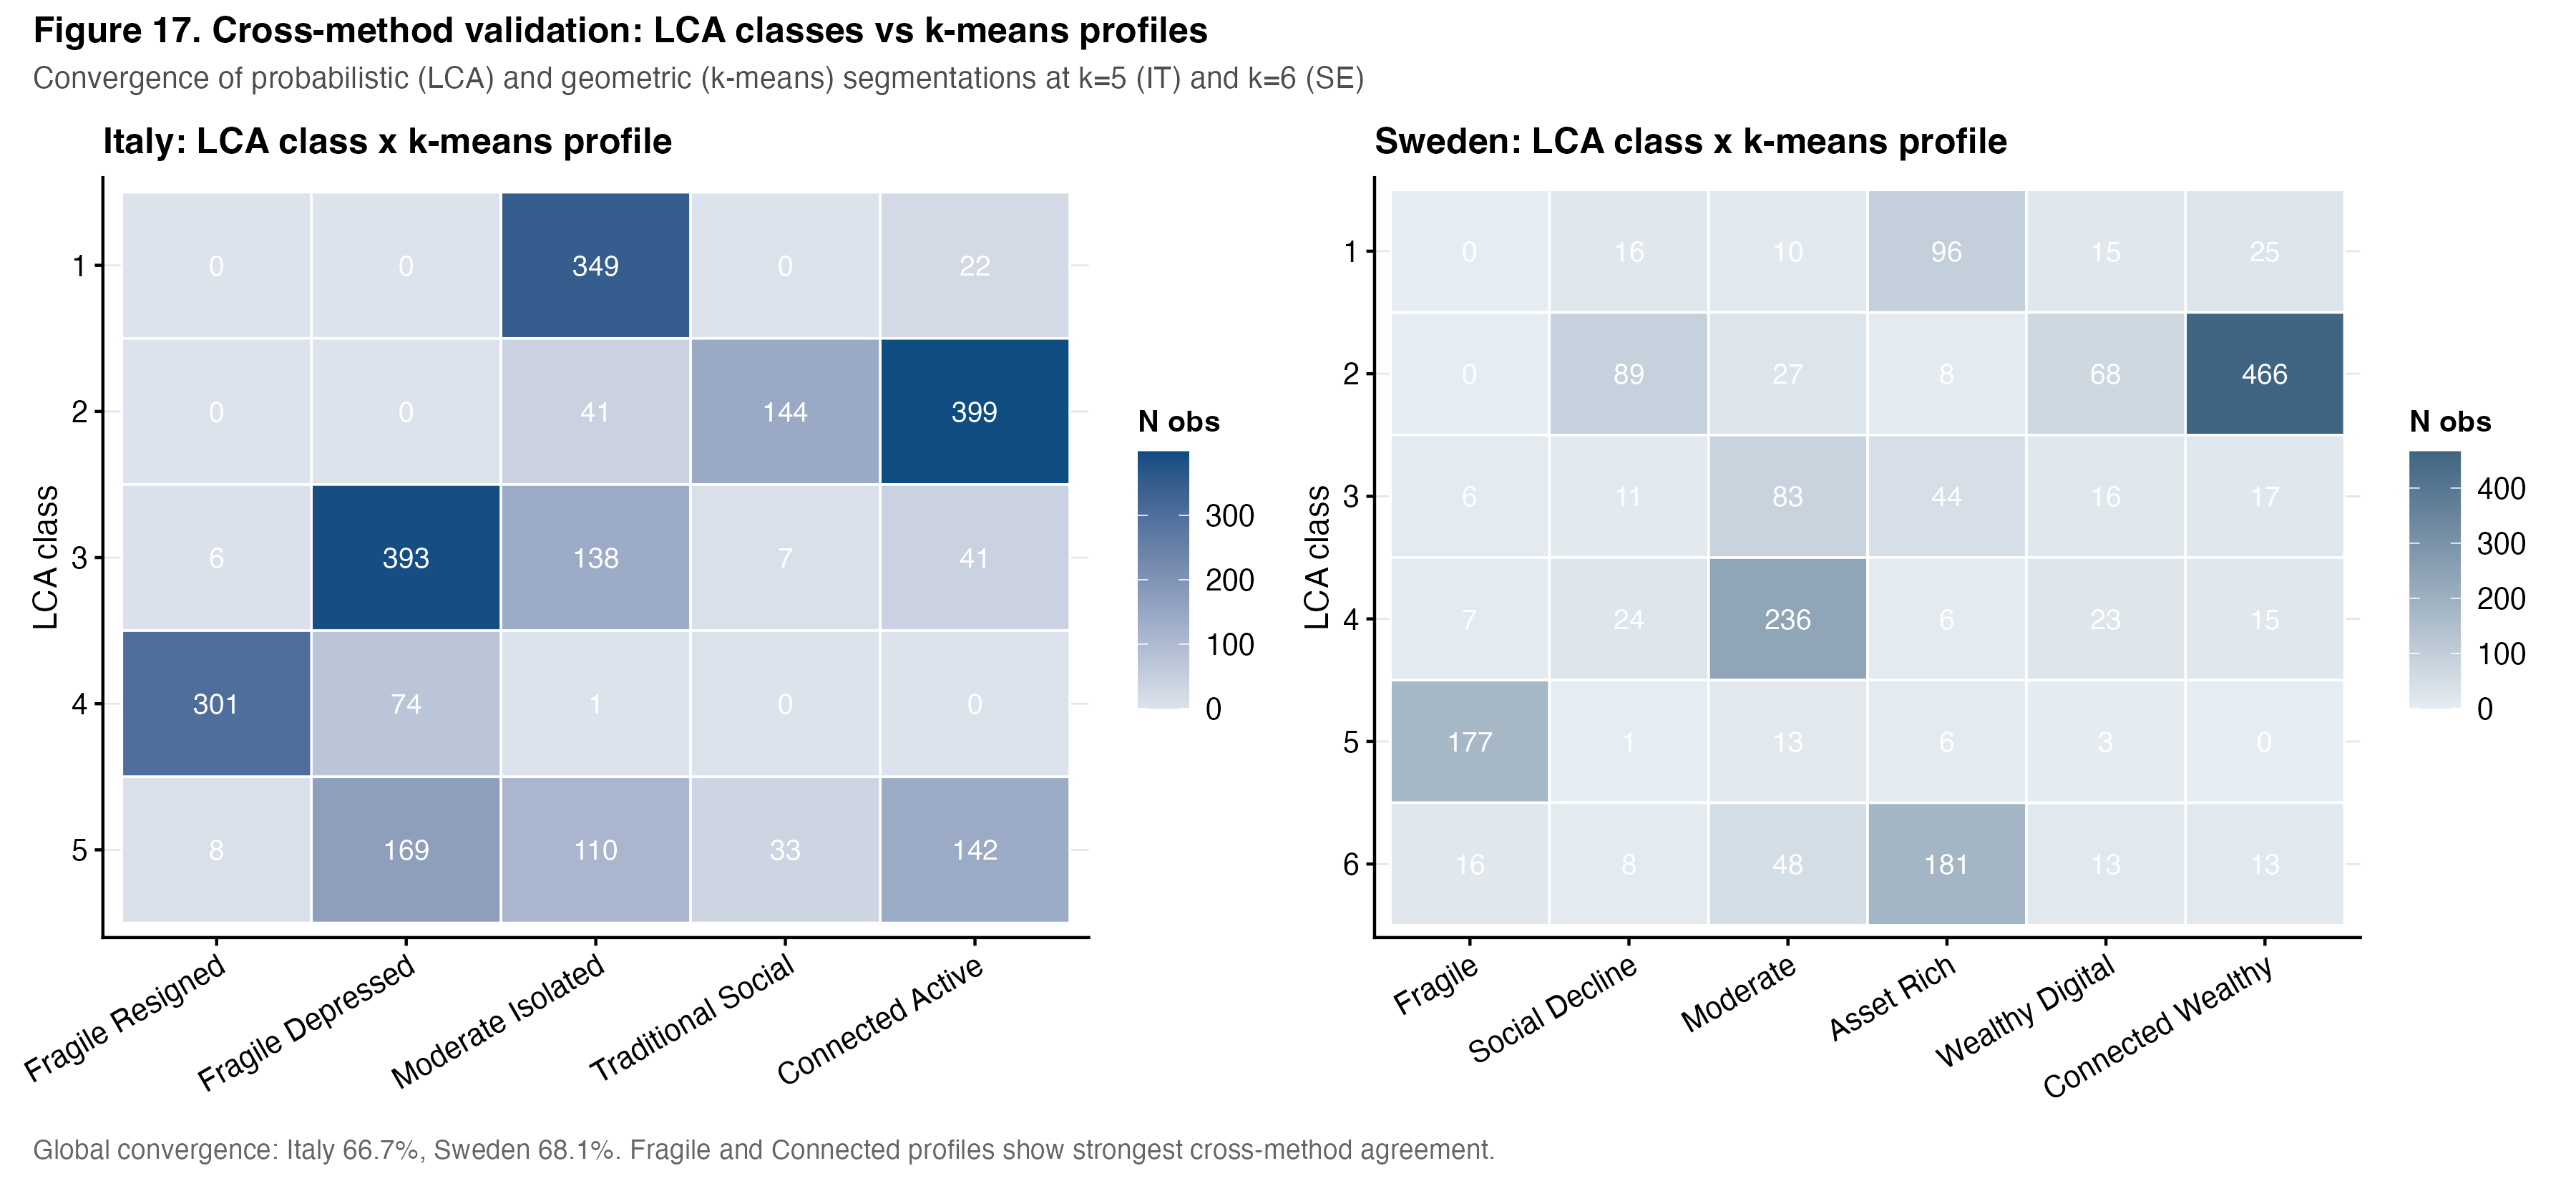
\includegraphics[width=0.85\linewidth]{figures/07_robustness/fig_17_lca_kmeans_confusion.png}
  \caption{Confusion between K-means profiles and LCA modal classes, by country. Source: v9 pipeline.}
  \label{fig:ch6-lca-confusion}
\end{figure}

\begin{figure}[ht]
  \centering
  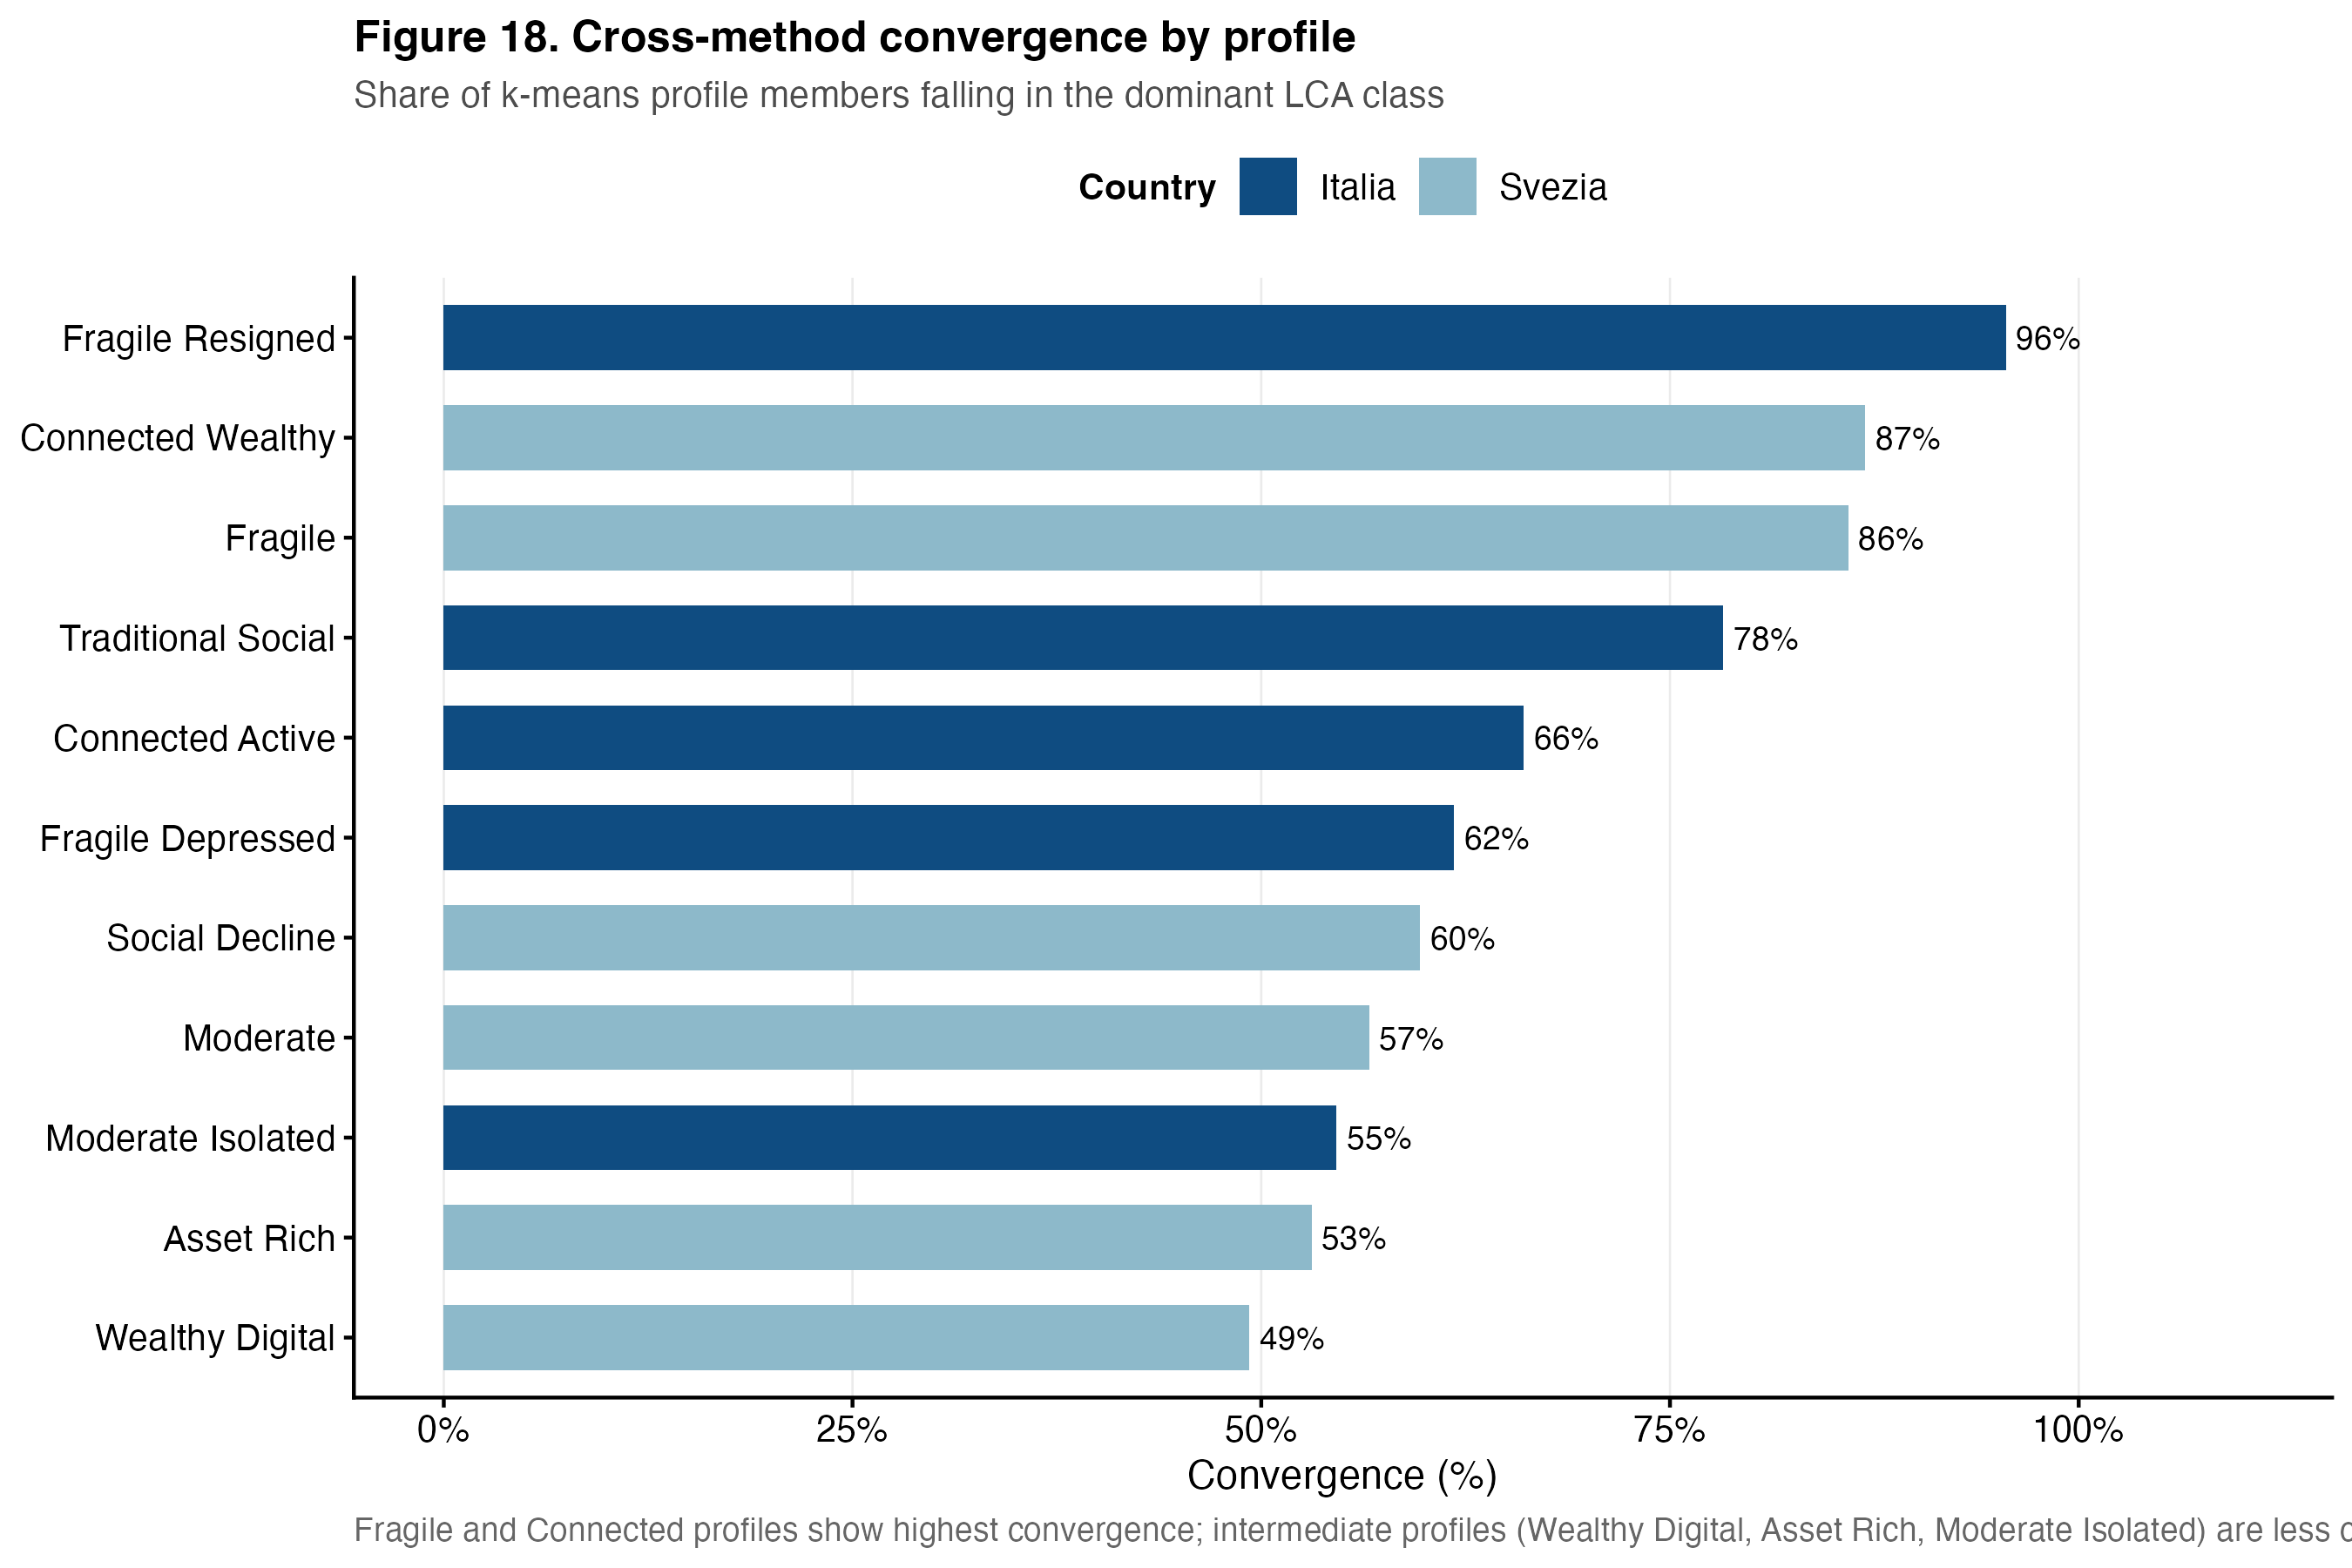
\includegraphics[width=0.78\linewidth]{figures/07_robustness/fig_18_convergence_per_profile.png}
  \caption{Profile-specific convergence between K-means and LCA. Source: v9 pipeline.}
  \label{fig:ch6-convergence}
\end{figure}

The profile-level pattern of Figure~\ref{fig:ch6-convergence} reveals two substantively interesting features. First, the Connected Active / Connected Wealthy profiles converge at rates above 70\% in both countries, indicating that the "connected upper tail" of each distribution is a robust latent type whose identification does not depend on the choice of clustering algorithm. Second, the Italian Fragile Resigned and Fragile Depressed profiles split across different LCA classes: this is not a failure of convergence but a confirmation that the subjective-block distinction between the two Fragile profiles is genuine and survives the probabilistic re-estimation.

Table~\ref{tab:ch6-lca-convergence} reports the profile-level convergence rate, computed as the share of members of a given K-means profile that are assigned to the modal LCA class.

\begin{table}[ht]
  \centering
  \caption{K-means--LCA convergence rate per profile.}
  \label{tab:ch6-lca-convergence}
  \small
  \begin{tabular}{@{}llrrr@{}}
    \toprule
    \textbf{Country} & \textbf{Profile} & \textbf{n} & \textbf{Modal LCA class} & \textbf{Convergence (\%)}\\
    \midrule
    Italy  & Fragile Resigned    & 315 & 4 & 95.6\\
    Italy  & Traditional Social  & 184 & 2 & 78.3\\
    Italy  & Connected Active    & 604 & 2 & 66.1\\
    Italy  & Fragile Depressed   & 636 & 3 & 61.8\\
    Italy  & Moderate Isolated   & 639 & 1 & 54.6\\
    \midrule
    Sweden & Connected Wealthy   & 536 & 2 & 86.9\\
    Sweden & Fragile             & 206 & 5 & 85.9\\
    Sweden & Social Decline      & 149 & 2 & 59.7\\
    Sweden & Moderate            & 417 & 4 & 56.6\\
    Sweden & Asset Rich          & 341 & 6 & 53.1\\
    Sweden & Wealthy Digital     & 138 & 2 & 49.3\\
    \bottomrule
  \end{tabular}
\end{table}

Three features of Table~\ref{tab:ch6-lca-convergence} deserve comment. First, the "pure" profiles at the extremes of the distribution are the most robust: \emph{Fragile Resigned} in Italy converges at 95.6\%, \emph{Connected Wealthy} in Sweden at 86.9\%, and the Swedish \emph{Fragile} at 85.9\%. Where the profile occupies an unambiguous position in the variable space, the probabilistic re-estimation reproduces the geometric assignment almost exactly. Second, the middle-range profiles converge at rates between 54\% and 66\% --- high enough to indicate a substantive latent type, but low enough to flag that the boundaries between adjacent profiles are soft. This is particularly true of the Italian \emph{Moderate Isolated} (54.6\%) and \emph{Fragile Depressed} (61.8\%), which share the subjective-block shadow that the 4D sensitivity analysis of Section~\ref{sec:ch6-subjective} dismantles. Third, the Swedish \emph{Wealthy Digital} and \emph{Asset Rich} profiles converge at rates just below 50\% and just above 53\% respectively: these are the two Swedish welfare-regime-specific types that Chapter~\ref{ch:ch5} flagged as unmatched, and their lower LCA convergence is consistent with their interpretive role as composite signatures of the universalist regime rather than crystallised latent types.

\section{Factor-solution stability}
\label{sec:ch6-fa-stability}

The six-factor PA-varimax solution is re-estimated on the pooled sample and, separately, on each country, to test whether the latent structure is stable across the two populations. Figure~\ref{fig:ch6-communalities} compares communalities of the 31 variables in Italy and Sweden; most variables have $h^{2}$ within $\pm 0.10$ across the two countries, with two notable exceptions. The first is \emph{social\_integration} in Sweden, whose Heywood case (loading $1.11$, $h^{2} = 1.38$) was flagged in Section~\ref{sec:ch3-fa}; the second is \emph{ac035d4} and \emph{ac035d7}, which in Italy have zero variance and are therefore absent from the Italian factor computation.

\begin{figure}[ht]
  \centering
  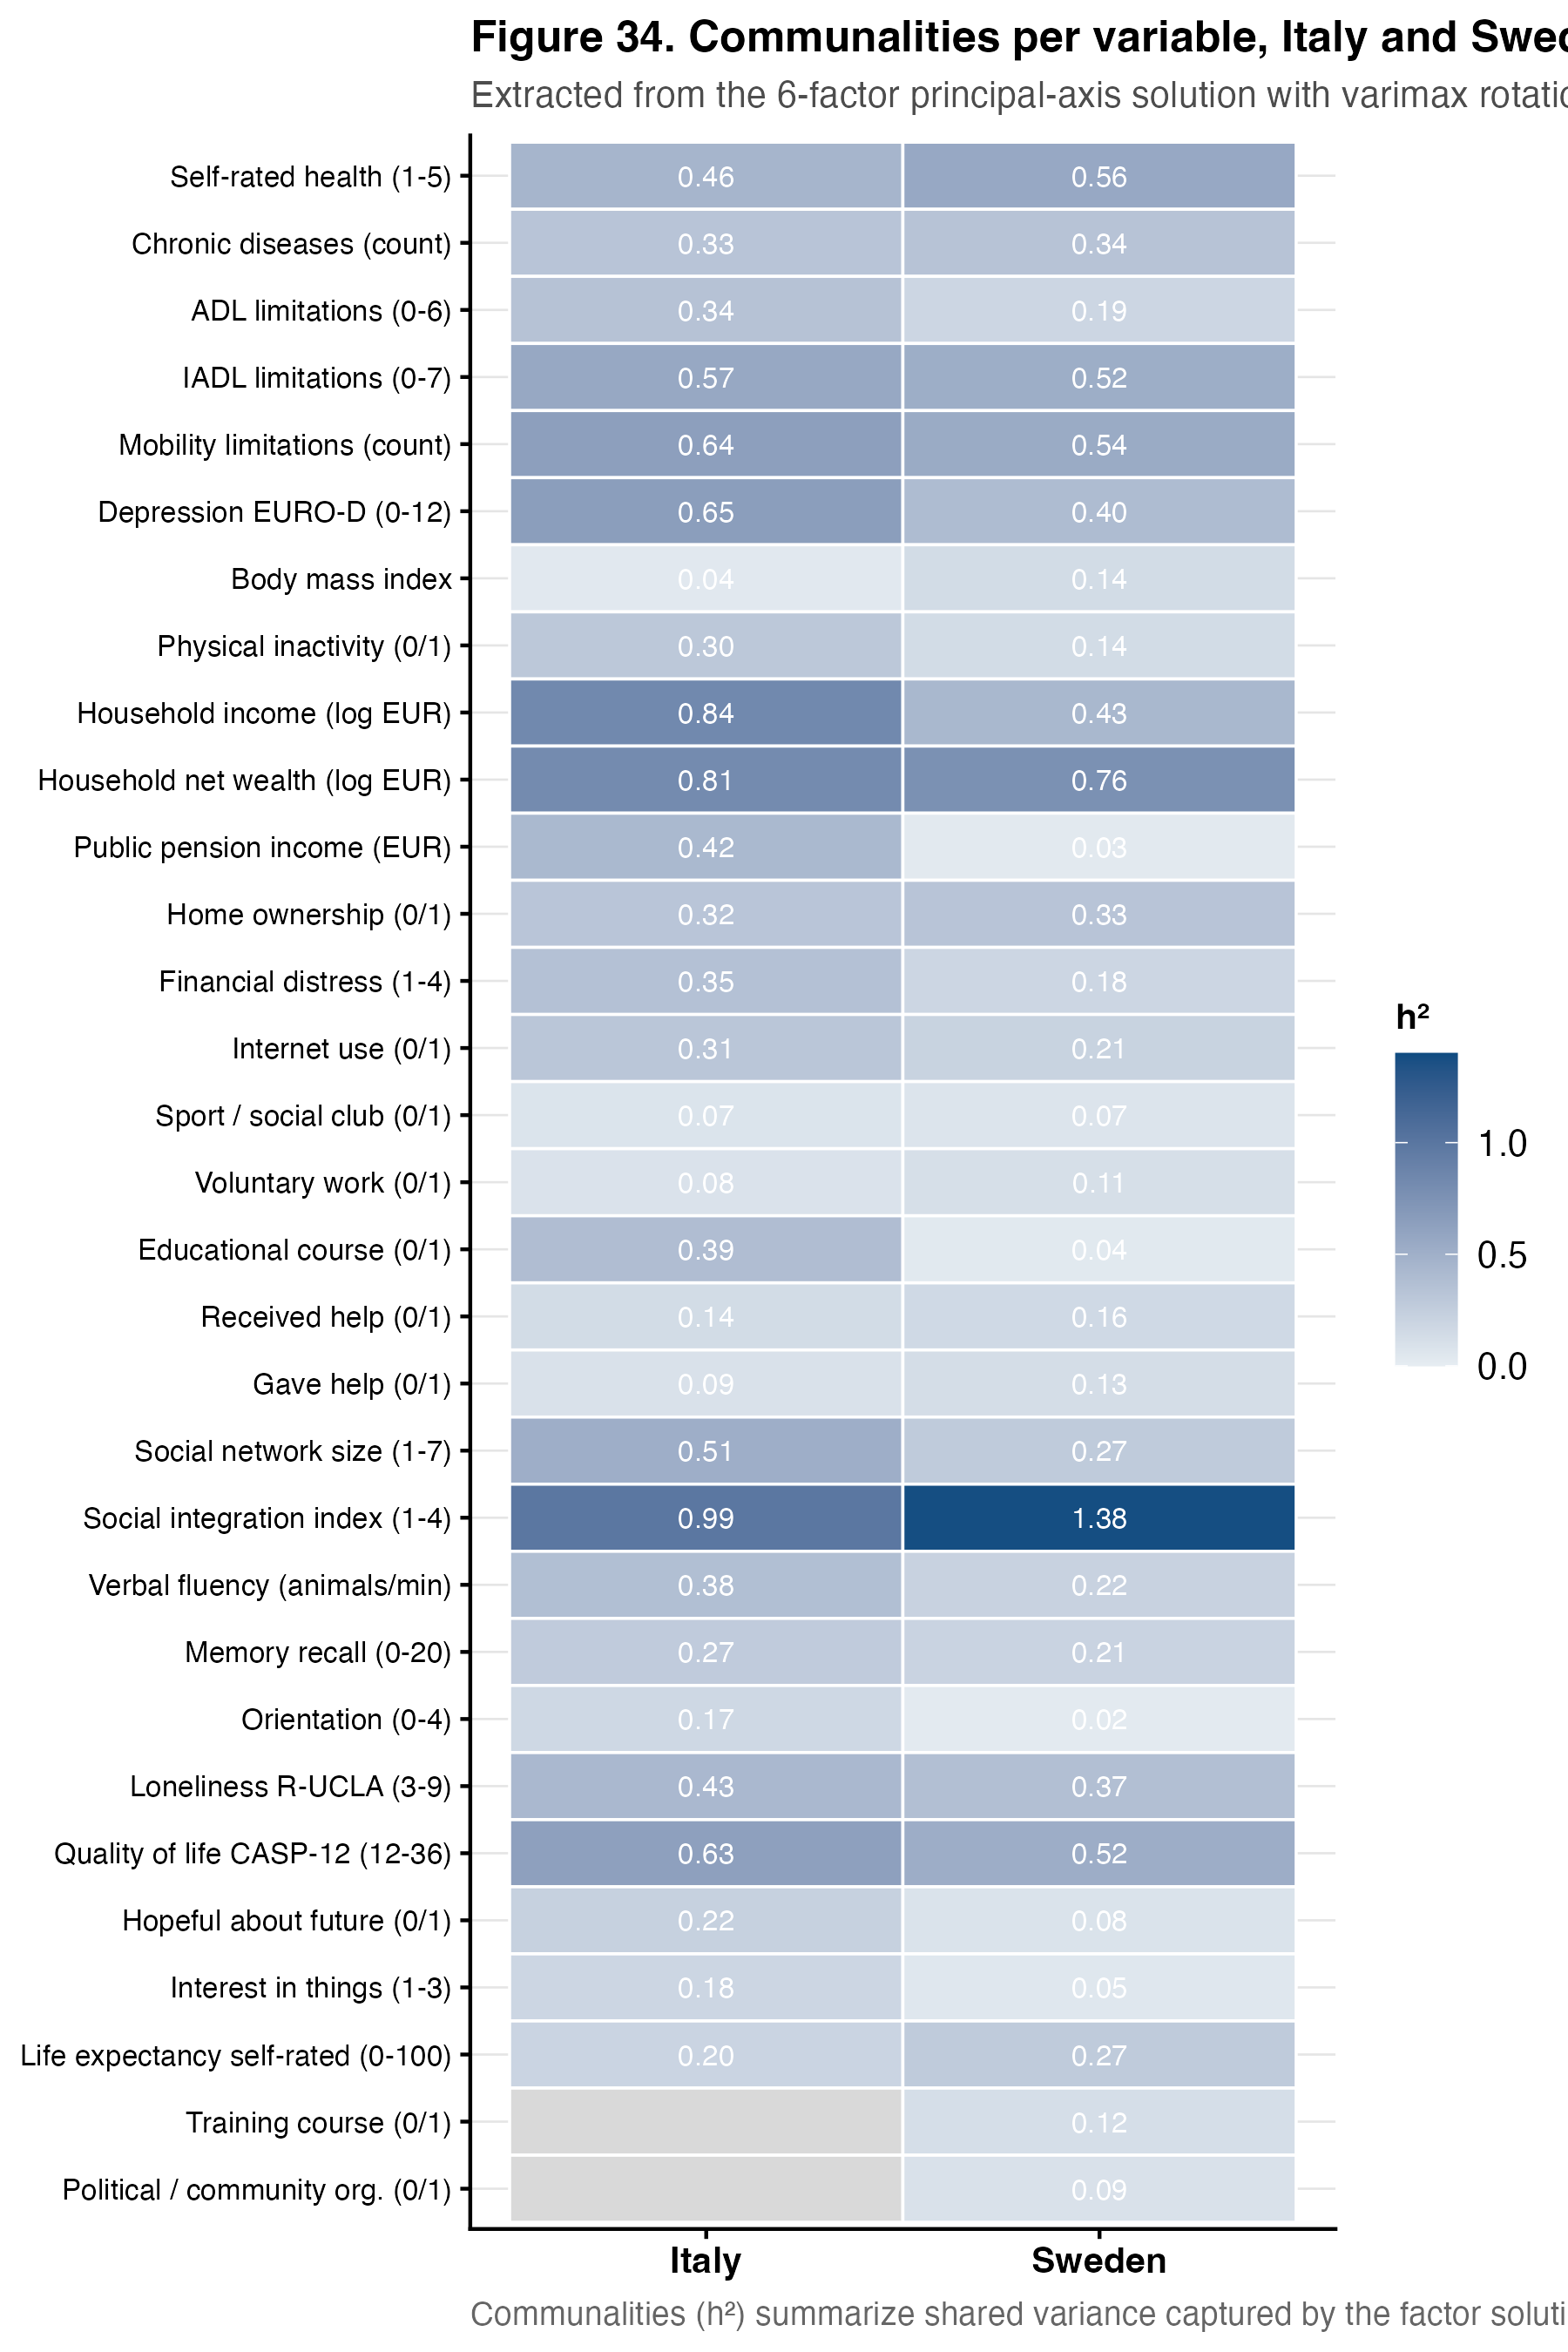
\includegraphics[width=0.70\linewidth]{figures/06_comparison/fig_34_communalities_heatmap.png}
  \caption{Communalities per variable, Italy and Sweden. Source: v9 pipeline.}
  \label{fig:ch6-communalities}
\end{figure}

Figure~\ref{fig:ch6-fa-fit} shows that the fit of the FA solution stabilises in the $k = 6$ region for both countries, consistent with the BIC-minimal range identified by parallel analysis. The Heywood case on \emph{social\_integration} is a known fragility of the Swedish specification and was the primary reason for choosing to cluster on the original standardised variables rather than on factor scores: this choice insulates the clustering stage from the instability of a single factor loading above one.

\begin{figure}[ht]
  \centering
  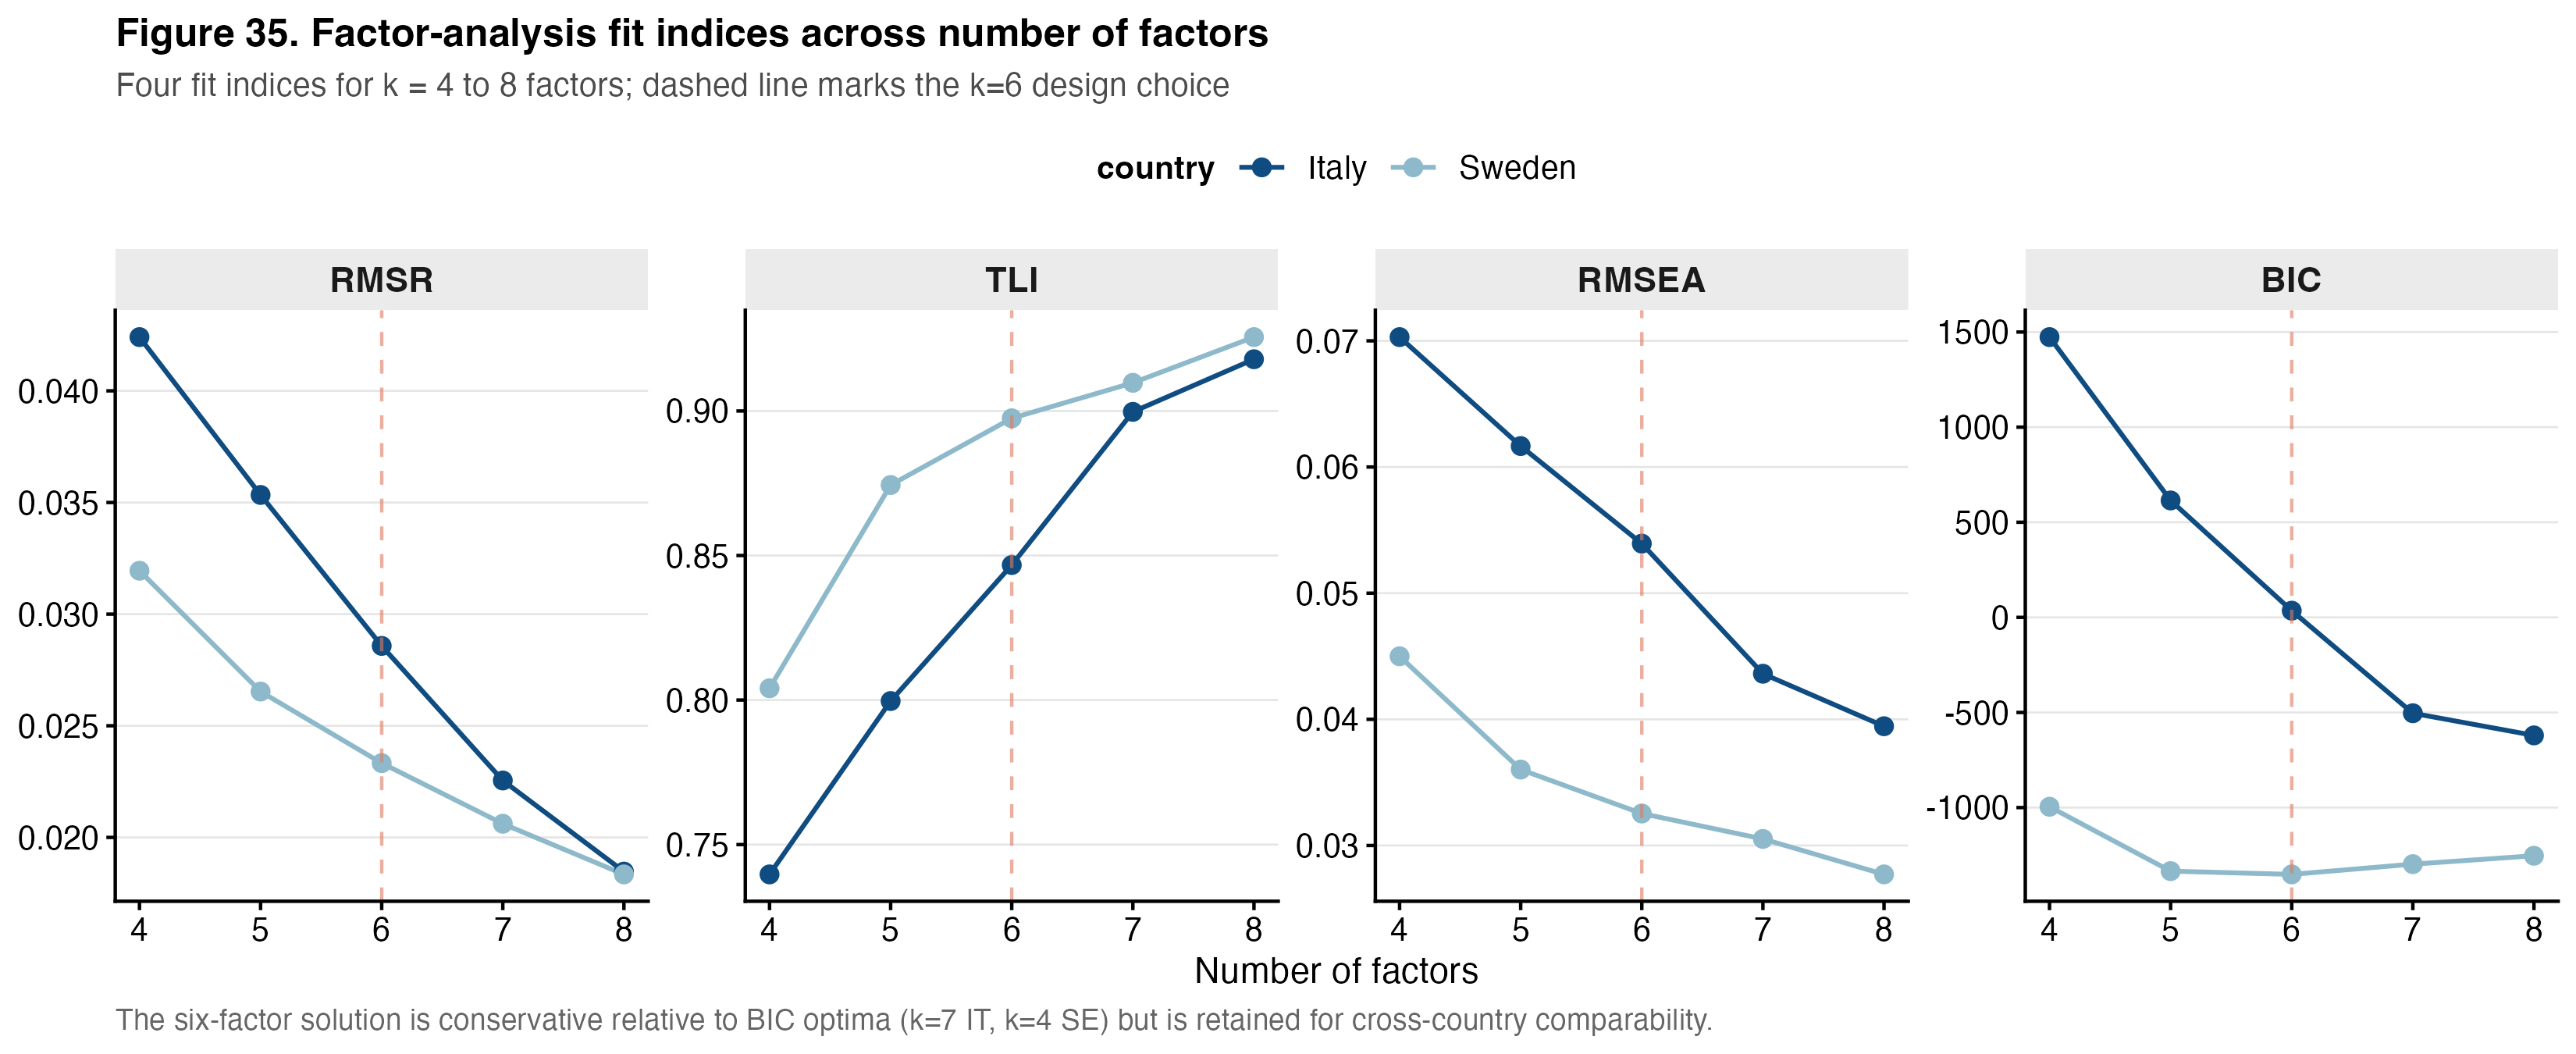
\includegraphics[width=0.75\linewidth]{figures/06_comparison/fig_35_fa_fit_comparison.png}
  \caption{FA fit comparison across $k = 4,\ldots,8$ factors, Italy and Sweden. Source: v9 pipeline.}
  \label{fig:ch6-fa-fit}
\end{figure}

\section{Sensitivity to the subjective block}
\label{sec:ch6-subjective}

The most searching robustness check concerns the thesis's analytical innovation itself: the inclusion of the five subjective variables (\emph{loneliness}, \emph{casp}, \emph{hope\_future}, \emph{interest}, \emph{expect\_alive}) as clustering inputs, rather than as external validation outcomes. If the identified profiles survived the removal of the subjective block essentially unchanged, the analytical innovation would be empirically vacuous; conversely, if the 4D solution collapsed a substantively important distinction that the 5D solution preserves, the innovation would be validated.

The 4D solution is fit by re-running K-means on the same pre-processing pipeline but dropping the five subjective variables, leaving 24 active variables in Italy and 26 in Sweden. $k$ is held fixed at 5 and 6, respectively, to make the comparison cleanest. Table~\ref{tab:ch6-sensitivity} reports four diagnostics: silhouette width, within-cluster $R^{2}$, the ANOVA $F$-statistic on life satisfaction (an indicator that does \emph{not} enter either specification and therefore serves as an impartial external validator), and the adjusted Rand index between the 4D and the 5D partitions.

\begin{table}[ht]
  \centering
  \caption{Sensitivity analysis: 4D vs 5D specification.}
  \label{tab:ch6-sensitivity}
  \small
  \begin{tabular}{@{}llrrrrr@{}}
    \toprule
    \textbf{Country} & \textbf{Specification} & \textbf{$k$} & \textbf{Silhouette} & \textbf{Within $R^{2}$} & \textbf{ANOVA $F$ on lifesat} & \textbf{ARI vs 5D}\\
    \midrule
    Italy  & 5D (reference) & 5 & 0.069 & 0.248 & 124.6 & --- \\
    Italy  & 4D             & 5 & 0.089 & 0.264 &  73.8 & 0.409 \\
    Sweden & 5D (reference) & 6 & 0.060 & 0.211 &  44.3 & --- \\
    Sweden & 4D             & 6 & 0.079 & 0.229 &  34.6 & 0.517 \\
    \bottomrule
  \end{tabular}
  \par\smallskip
  \footnotesize \emph{Note.} 4D specification drops \emph{loneliness}, \emph{casp}, \emph{hope\_future}, \emph{interest} and \emph{expect\_alive} from the clustering input (24 active vars in Italy, 26 in Sweden). Life satisfaction is external to both specifications. ANOVA $F$ is $F(4, 2183)$ for Italy and $F(5, 1779)$ for Sweden. Adjusted Rand index (ARI) between 4D and 5D assignments is reported in the last column.
\end{table}

The interpretation of Table~\ref{tab:ch6-sensitivity} rests on three contrasts.

First, the silhouette and within-cluster $R^{2}$ are slightly \emph{higher} in the 4D specification than in the 5D reference (silhouette $0.089$ vs $0.069$ for Italy; $0.079$ vs $0.060$ for Sweden). This is expected: clustering on fewer variables produces tighter partitions in a reduced space, and no claim of robustness should rest on these metrics. The fact that the 4D solution looks "cleaner" by internal criteria is not an argument in its favour.

Second, the ANOVA $F$-statistic on life satisfaction --- which is external to both specifications and therefore impartial --- strongly favours the 5D solution. In Italy the 5D profiles produce $F = 124.6$ against the 4D's $F = 73.8$ (a 69\% reduction when the subjective block is removed). In Sweden the pattern is the same in direction though smaller in magnitude: $F = 44.3$ vs $F = 34.6$, a 28\% reduction. Since life satisfaction did not enter either clustering input, this is direct evidence that the 5D partitions discriminate lived well-being substantially better than the 4D partitions, despite their lower internal metrics. The 5D clustering identifies groups of individuals who differ systematically on a variable the clustering never saw; the 4D clustering, by dropping the subjective-block correlations, loses a third to a half of that discriminative power.

Third, the adjusted Rand index between the 4D and 5D partitions is $0.41$ for Italy and $0.52$ for Sweden. Values this far from one mean that the two specifications disagree on a substantial share of the assignments: roughly half of the Italian respondents and half of the Swedish ones fall in a different profile when the subjective block is removed. If the subjective variables had been redundant with the objective ones the ARI would approach unity.

The qualitative nature of the 4D--5D disagreement is most visible on the Italian cross-tabulation, reported in Table~\ref{tab:ch6-crosstab}. Three patterns emerge. First, \emph{Fragile Resigned} (95\% of its 315 members map to a single 4D cluster) and \emph{Traditional Social} (99\% of its 184 members map to a single 4D cluster) are the profiles whose identification does not depend on the subjective block: they are already separable on objective variables alone. Second, the substantive mixing is between \emph{Fragile Depressed} and \emph{Moderate Isolated}: the 4D cluster that contains the plurality of Fragile Depressed (cluster~2, 350 of its 636 members) also contains the plurality of Moderate Isolated (cluster~2, 345 of its 639 members). Without the subjective block, the 4D solution cannot distinguish a high-CASP, high-hope isolated profile from a low-CASP, depressed profile with the same objective conditions: they look alike, and they cluster together. Third, \emph{Connected Active} is mostly preserved in a single 4D cluster (cluster~5, 487 of 604 members) but sheds about a sixth of its members to the mixed Fragile-Depressed / Moderate-Isolated cluster~3.

\begin{table}[ht]
  \centering
  \caption{Italy: cross-tabulation of the 5D profile labels against the 4D cluster labels ($k = 5$).}
  \label{tab:ch6-crosstab}
  \small
  \begin{tabular}{@{}lrrrrr@{}}
    \toprule
    \textbf{5D profile $\backslash$ 4D cluster} & \textbf{1} & \textbf{2} & \textbf{3} & \textbf{4} & \textbf{5}\\
    \midrule
    Fragile Resigned     &   1 &   0 &   0 & 314 &   0\\
    Fragile Depressed    &   2 & 350 & 162 & 107 &  15\\
    Moderate Isolated    &   0 & 345 & 195 &   1 &  98\\
    Traditional Social   & 183 &   1 &   0 &   0 &   0\\
    Connected Active     &   0 &   4 & 103 &  10 & 487\\
    \bottomrule
  \end{tabular}
  \par\smallskip
  \footnotesize \emph{Note.} Cells report the number of Italian respondents assigned to each combination. The 4D cluster that collapses Fragile Depressed and Moderate Isolated (cluster~2) is the empirical signature of the claim that the subjective block is not redundant with the objective variables.
\end{table}

Taken together, Tables~\ref{tab:ch6-sensitivity} and~\ref{tab:ch6-crosstab} support the analytical choice of including the subjective block as a clustering input. Removing it produces a partition that is marginally tighter by internal metrics but loses substantial external discriminative power on life satisfaction, disagrees with the 5D solution on about half of the assignments, and --- most importantly --- collapses the Fragile Depressed / Moderate Isolated contrast that is the substantive hinge of Chapter~\ref{ch:ch7}. The case for the 5D specification is thus established not by its superior fit but by the interpretability of the additional structure it preserves.

\section{Chapter summary}
\label{sec:ch6-summary}

Across five independent robustness checks --- multi-algorithm cluster-quality comparison, Duda--Hart cut-off diagnostics, K-means / LCA convergence, factor-solution stability, and the 4D vs 5D sensitivity analysis --- the five Italian and six Swedish profiles survive re-estimation under alternative methodological choices. The principal vulnerability of the segmentation is the Heywood case on the Swedish social-integration index, discussed in Section~\ref{sec:ch6-fa-stability}, which motivated the decision (already taken in Section~\ref{sec:ch3-kmeans}) to cluster on standardised original variables rather than on factor scores. The most substantively important check is Section~\ref{sec:ch6-subjective}: removing the subjective block from the clustering input collapses the Fragile Depressed / Moderate Isolated contrast that the 5D solution preserves, reduces the external ANOVA $F$-statistic on life satisfaction by roughly a third to a half, and produces a partition that disagrees with the 5D reference on about half of the assignments (ARI $= 0.41$ in Italy, $0.52$ in Sweden). This is the empirical basis for the thesis's claim that the subjective block is not redundant with the objective variables and earns its place as a clustering input, and it is also the statistical foundation for the substantive argument of Chapter~\ref{ch:ch7}, where the Moderate Isolated profile --- the one whose identification depends most critically on the subjective block --- turns out to pay a measurable cost in healthcare access.
